
% VLDB template version of 2020-08-03 enhances the ACM template, version 1.7.0:
% https://www.acm.org/publications/proceedings-template
% The ACM Latex guide provides further information about the ACM template

\documentclass[sigconf, nonacm]{acmart}

% \usepackage{cite}
% \usepackage{amsmath,amssymb,amsfonts}
\usepackage{algorithm2e}
\usepackage{graphicx}
\usepackage{textcomp}
\usepackage{subcaption}
\usepackage{balance}

% %%%%%%%%%%%---My Packages-----%%%%%%
% \usepackage{fancyhdr}
% \usepackage[normalem]{ulem}
% \usepackage[hyphens]{url}
% \usepackage[sort,nocompress]{cite}
% \def\baselinestretch{0.9}
% Always include hyperref last
% \usepackage[bookmarks=true,breaklinks=true,letterpaper=true,colorlinks,linkcolor=black,citecolor=blue,urlcolor=black]{hyperref}
\usepackage[binary-units=true]{siunitx}
% \sisetup{per-mode=symbol,per-symbol = /}
% \usepackage{mathtools}
\usepackage{booktabs}
% \usepackage[dvipsnames]{xcolor}
\usepackage{enumitem}
\usepackage[skip=2pt]{caption}
%%%%%%%%%%%%%%%%%%%%%%%%%%%%%%%%%%%%
%%%%%%%%%%%%---Math operators-----%%%%%%%%%%%
\DeclareMathOperator{\PR}{PR}
\DeclareMathOperator{\PRprime}{PR^\prime}
\DeclareMathOperator{\PRnext}{PR_{next}}
\DeclareMathOperator{\inNeighbors}{inNeighbors}
\DeclareMathOperator{\outDegree}{outDegree}
\DeclareMathOperator{\divClause}{divClause}
\DeclareMathOperator{\divClauseMin}{divClause_{min}}
\DeclareMathOperator{\divClauseMax}{divClause_{max}}
\DeclareMathOperator{\clampRange}{clamp_{range}}
\DeclareMathOperator{\rangMin}{Range_{min}}
\DeclareMathOperator{\rangMax}{Range_{max}}
\DeclareMathOperator*{\Sum}{\mathlarger{\sum}}
\DeclareMathOperator*{\SSum}{\mathlarger{\mathlarger{\mathlarger{\sum}}}}
%%%%%%%%%%%%%%%%%%%%%%%%%%%%%%%%%%%%%%%%%%%%%

%% The following content must be adapted for the final version
% paper-specific
\newcommand\vldbdoi{XX.XX/XXX.XX}
\newcommand\vldbpages{XXX-XXX}
% issue-specific
\newcommand\vldbvolume{19}
\newcommand\vldbissue{1}
\newcommand\vldbyear{2026}
% should be fine as it is
\newcommand\vldbauthors{\authors}
\newcommand\vldbtitle{\shorttitle} 
% leave empty if no availability url should be set
\newcommand\vldbavailabilityurl{https://github.com/atmughrabi/GraphBrew}
% whether page numbers should be shown or not, use 'plain' for review versions, 'empty' for camera ready
\newcommand\vldbpagestyle{plain} 

\begin{document}
\title{GraphBrew: Multilayered Graph Reordering for Accelerated Graph Processing}

%%
%% The "author" command and its associated commands are used to define the authors and their affiliations.
\author{Abdullah T. Mughrabi}
\affiliation{%
  \institution{Department of Computer Science, University of Virginia}
  \city{Charlottesville}
  \state{Virginia}
  \country{USA}
}
\email{atmughra@virginia.edu}
\email{atmughra@alumni.ncsu.edu}

\author{Mohannad M. Ibrahim}
\affiliation{%
  \institution{Department of Electrical and Computer Engineering, North Carolina State University}
  \city{Raleigh}
  \state{North Carolina}
  \country{USA}
}
\email{mmibrah2@alumni.ncsu.edu}

\author{Morteza Baradaran}
\affiliation{%
  \institution{Department of Computer Science, University of Virginia}
  \city{Charlottesville}
  \state{Virginia}
  \country{USA}
}
\email{rgq5aw@virginia.edu}

\author{Beenish Gul}
\affiliation{%
  \institution{Department of Computer Science, University of Virginia}
  \city{Charlottesville}
  \state{Virginia}
  \country{USA}
}
\email{bg9qq@virginia.edu}


\author{Gregory T. Byrd}
\affiliation{%
  \institution{Department of Electrical and Computer Engineering, North Carolina State University}
  \city{Raleigh}
  \state{North Carolina}
  \country{USA}
}
\email{gbyrd@ncsu.edu}

\author{Kevin Skadron}
\affiliation{%
  \institution{Department of Computer Science, University of Virginia}
  \city{Charlottesville}
  \state{Virginia}
  \country{USA}
}
\email{skadron@virginia.edu}
%%
%% The abstract is a short summary of the work to be presented in the
%% article.
\begin{abstract}
Graph algorithms suffer from random fine-grain memory access patterns that cause low temporal and spatial cache locality. A widely used mitigation strategy is to reorder (relabel) graph vertices based on their inherent clustering and degree properties. Although reordering improves per-iteration execution time through better caching, it adds significant overhead to end-to-end graph processing, especially for dynamic graphs that are constantly updated. This overhead motivates lightweight reordering techniques that incorporate fewer graph structure features---such as degree-based grouping or community labeling---achieving faster preprocessing but with suboptimal cache performance.

A key observation, however, is that \emph{no single reordering technique is universally optimal}: the best strategy depends on both the graph topology (e.g., power-law social networks vs.\ mesh-like road graphs) and the algorithm's access pattern (iterative vs.\ traversal, pull vs.\ push). Prior lightweight techniques fail to account for this diversity, delivering fixed strategies that underperform on certain graph--algorithm pairs.

We introduce GraphBrew, a composable multilayered reordering framework that addresses this challenge. GraphBrew decomposes the reordering problem into pluggable stages---community detection, intra-community ordering, and inter-community arrangement---each targeting a distinct locality dimension. By combining these stages in different configurations, GraphBrew provides nine reordering variants along with chained multi-stage orderings, each tailored to specific graph topologies and algorithm access patterns. Our systematic evaluation across diverse graph topologies and algorithms demonstrates that GraphBrew variants achieve cache miss rates comparable to the state-of-the-art Gorder while requiring up to $6\times$ less reordering time. We further show that different variants excel on different graph--algorithm pairs, validating the need for a composable reordering framework rather than a monolithic solution.
\end{abstract}

\maketitle

%%% do not modify the following VLDB block %%
%%% VLDB block start %%%
\pagestyle{\vldbpagestyle}
\begingroup\small\noindent\raggedright\textbf{PVLDB Reference Format:}\\
\vldbauthors. \vldbtitle. PVLDB, \vldbvolume(\vldbissue): \vldbpages, \vldbyear.\\
\href{https://doi.org/\vldbdoi}{doi:\vldbdoi}
\endgroup
\begingroup
\renewcommand\thefootnote{}\footnote{\noindent
This work is licensed under the Creative Commons BY-NC-ND 4.0 International License. Visit \url{https://creativecommons.org/licenses/by-nc-nd/4.0/} to view a copy of this license. For any use beyond those covered by this license, obtain permission by emailing \href{mailto:info@vldb.org}{info@vldb.org}. Copyright is held by the owner/author(s). Publication rights licensed to the VLDB Endowment. \\
\raggedright Proceedings of the VLDB Endowment, Vol. \vldbvolume, No. \vldbissue\ %
ISSN 2150-8097. \\
\href{https://doi.org/\vldbdoi}{doi:\vldbdoi} \\
}\addtocounter{footnote}{-1}\endgroup
%%% VLDB block end %%%

%%% do not modify the following VLDB block %%
%%% VLDB block start %%%
\ifdefempty{\vldbavailabilityurl}{}{
\vspace{.3cm}
\begingroup\small\noindent\raggedright\textbf{PVLDB Artifact Availability:}\\
The source code, data, and/or other artifacts have been made available at \url{\vldbavailabilityurl}.
\endgroup
}
%%% VLDB block end %%%


\section{Introduction}
Graph analytics are prevalent in many domains, playing an essential role in social networks, biomedical sciences, and graph neural networks (GNNs) \cite{ang_introducing_2010,lee_extrav_2017,zhou_graph_2019}. The broad adoption of graph processing is due to graph data structures presenting a powerful abstraction that streamlines algorithm implementations. However, performance challenges arise from a high ratio of random fine-grain memory accesses across large data sets, overwhelming the target system bandwidth and causing high cache miss rates \cite{lumsdaine_challenges_2007,beamer_locality_2015,beamer_reducing_2017,wei_speedup_2016}.

\begin{figure}[t]
  \centering
  
\includegraphics[width=\linewidth]{paperFigures/Fig3}
  \caption{Graph representation in CSR format. Vertex data accesses are non-sequential and fine-grained, leading to a high cache miss rate.}
  \label{fig:fig3}
\end{figure}

Fig.~\ref{fig:fig3} illustrates a conventional graph processing approach in shared memory systems, known as a vertex-centric \cite{mccune_thinking_2015} or a Gather-Apply-Scatter (GAS) model. As shown in Algorithm~\ref{algo:fig2}, the vertex-centric approach employs a Compressed Sparse Row (CSR) matrix data structure to represent the graph in memory for easy neighbor access. While visiting neighbors for each vertex in a streamlined manner might seem intuitive with the GAS model, the scattering of neighbor IDs across memory generates irregular access patterns, leading to low spatial and temporal locality with a high cache miss rate.

\begin{algorithm}[b]
	\SetAlgoLined
	\leftline{
\includegraphics[width=0.7\linewidth]{paperFigures/Fig2}}
	\caption{Graph traversal, with CSR structure.}
	\label{algo:fig2}
\end{algorithm}

One key characteristic of graph vertices is their \emph{power-law} or skewed degree distribution \cite{barabasi_scale-free_2009,zhang_making_2017,balaji_when_2018,faloutsos_power-law_1999,beamer_gap_2017,zhang_optimizing_2016}. \emph{Power-law} graphs exhibit a topology where a small percentage of vertices hold the majority of connections. Such graphs are prevalent in applications like social networks and are often noted as \emph{scale-free} or \emph{natural} graphs.
The internal labeling of vertices can also contribute to a bottleneck during graph traversal. For instance, a vertex-centric algorithm propagates from a source vertex through its neighbors, as shown in Algorithm~\ref{algo:fig2}. Among the many factors affecting traversal performance, a key one is how the data accessed within and across graph community clusters are spatially and temporally coalesced.

Previous research has demonstrated cache optimization techniques for better bandwidth utilization through reordering vertex IDs \cite{arai_rabbit_2016,balaji_when_2018,balaji_combining_2019,faldu_closer_2020,wei_speedup_2016}. Such techniques exploit graph skewness and clustering to improve cache reuse between a vertex and its neighbors across the graph data arrays. The fundamental trade-off is between the sophistication of the reordering analysis and its overhead. Fig.~\ref{fig:fig1} shows an approximation of the end-to-end performance with different reordering techniques. Generally, more sophisticated analysis techniques lead to better cache locality and performance, but the cost of performing the analysis leads to higher end-to-end latency. Pre-processing time \cite{malicevic_everything_2017}, which includes reading the graph edge-list from the file and building the CSR structure as demonstrated in Fig.~\ref{fig:fig3}, is increased with a reorder step. Consequently, the higher overhead of sophisticated reordering techniques may not be overcome by the improved cache performance, leading to longer end-to-end latency.

This study introduces GraphBrew, a novel composable multilevel lightweight reordering framework. Rather than proposing a single fixed strategy, GraphBrew decomposes the reordering problem into pluggable stages---community detection, intra-community ordering, and inter-community arrangement---each targeting a distinct locality dimension. By combining these stages in different configurations, GraphBrew offers nine distinct reordering variants along with chained multi-stage orderings. The framework builds upon established lightweight techniques such as Leiden community detection \cite{traag_louvain_2019}, Rabbit Order \cite{arai_rabbit_2016}, and Degree Based Grouping (DBG) \cite{faldu_closer_2020}, composing them in novel multilayered configurations. Each variant maintains the low overhead of lightweight reordering while achieving cache performance comparable to state-of-the-art Gorder \cite{wei_speedup_2016}. We detail all nine variants in Section~\ref{sec:multilayer}.

Our main contributions in this paper are summarized as follows:
\begin{itemize}[topsep=2pt,itemsep=2pt,wide]
\item We demonstrate that no single reordering technique is universally optimal by evaluating cache performance across diverse graph topologies (social, web, road, citation) and algorithms (iterative, traversal, pull-based, push-based), showing that the best reordering strategy depends on both graph structure and algorithm access pattern.
\item We introduce GraphBrew, a composable multilayered reordering framework with nine pluggable variants along with chained multi-stage orderings that enable fine-grained control over the reordering pipeline (Section~\ref{sec:multilayer}).
\item We present a systematic evaluation of all GraphBrew variants across a diverse set of graph structures and algorithms, contrasting them against established baselines including DBG, Rabbit Order, Gorder, RCM, and GoGraph.
\item We provide a variant ablation study demonstrating the contribution of each composable layer and a graph-type sensitivity analysis showing which variants excel on which graph topologies.
\item We release GraphBrew as an open-source reproducible benchmark framework with automated experiment scripts for the community.
\end{itemize}

 \begin{figure}[b]
  \centering
  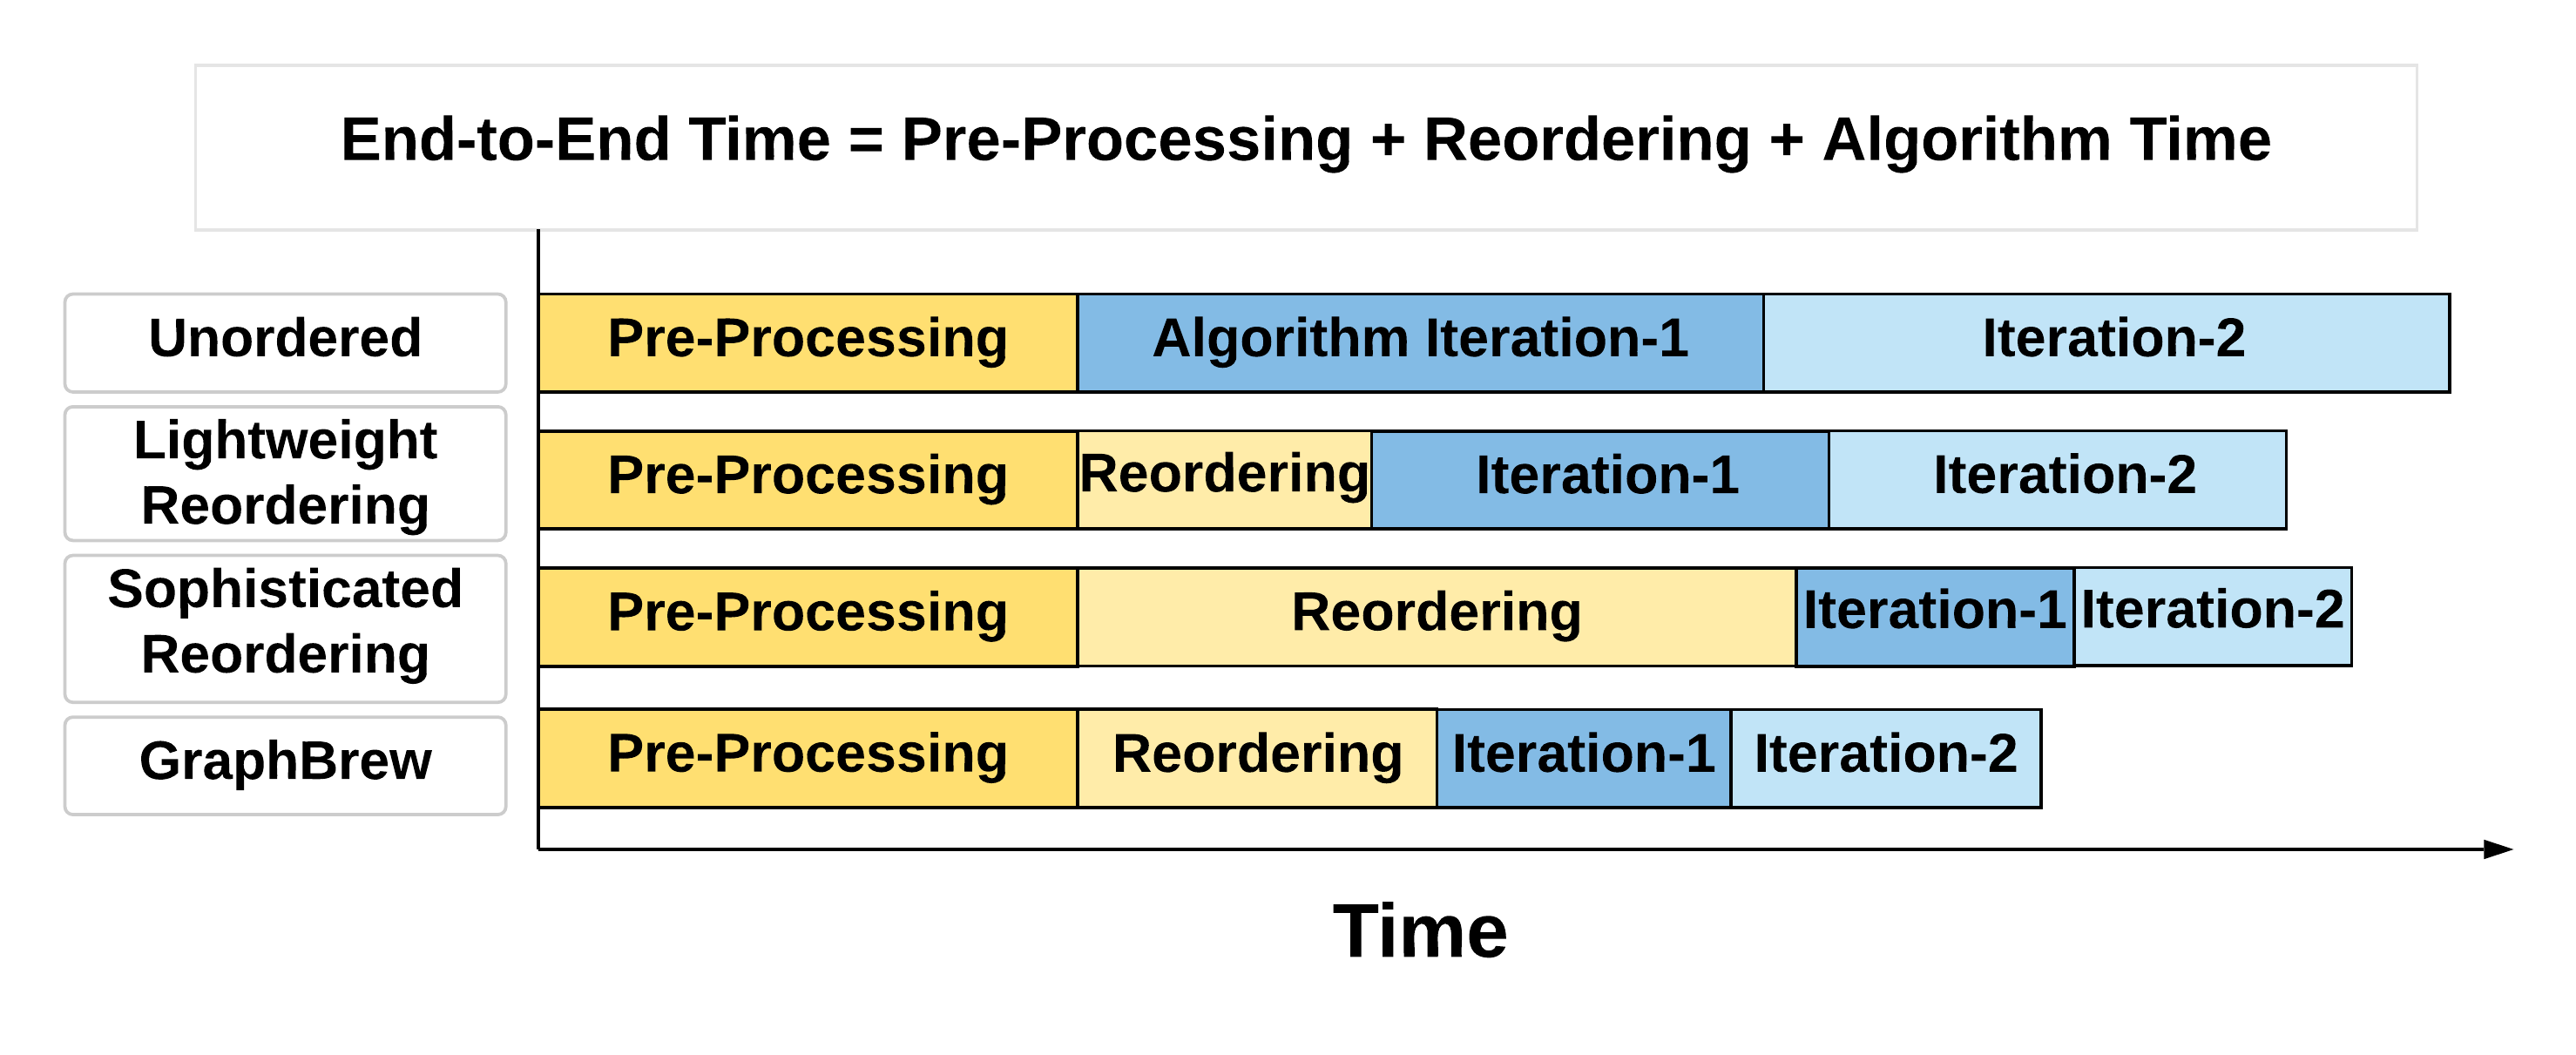
\includegraphics[width=\linewidth]{paperFigures/Fig1c}
  \caption{Graph pre-processing overhead trade-offs. Reordering can improve algorithm performance but increases end-to-end execution time.}
  \label{fig:fig1}
\end{figure}

\section{Background}
\label{sec:background}

\subsection{Graph Processing Model}
\label{sec:processing_model}
Graph algorithm access patterns usually fall into a few well-known categories. Understanding these categories is essential for explaining why graph algorithm performance suffers from irregular memory access patterns with high cache miss ratios. A growing body of literature \cite{beamer_direction-optimizing_2012, besta_push_2017} characterizes these behavioral patterns for vertex-centric graph algorithms operating on CSR data structures:

\begin{itemize}[topsep=2pt,itemsep=2pt,wide]
\item \textbf{Iterative:} An iterative graph algorithm processes all the graph vertices in each iteration until reaching a convergence criterion. This behavior often requires a cache that fits the whole graph dataset for fewer capacity misses and less thrashing. Iterative algorithms can benefit from reordering, with each community \cite{arai_rabbit_2016} within the graph labeled closely together for better scheduling when looping within each iteration and reading the graph data arrays \cite{mukkara_exploiting_2018}. Good examples of iterative algorithms are PageRank (PR) and Sparse Matrix-Vector Multiplication (SpMV).
\item \textbf{Traversal:} A traversing algorithm typically starts from a source vertex and propagates through the vertex neighbors in a frontier manner through the graph. Each traversal activates the neighboring vertices in the frontier. Such behavior often requires caching the active vertices set within a graph community on frontier traversal bases. Furthermore, there is a high probability of visiting high degree vertices in the graph within each traversal, giving the incentive to reorder according to the graph degree skewness. Good examples of traversal algorithms are Breadth-First Search (BFS), Single Source Shortest Path (SSSP), and Connected Components (CC).
\item \textbf{Pull-Based:} The pull-based approach describes data propagation between vertices in the processed graph. With a pull-based graph algorithm, the processed vertex gathers data from neighboring vertices while updating itself. This technique is effective in parallel implementation of graph algorithms where each core is scheduled a single vertex in parallel, eliminating the need for locks \cite{besta_push_2017}. Relabeling graph vertices in pull-based algorithms requires grouping hot (frequently-used) vertices based on their out-degree for better caching. For instance, vertices with higher out-degree have a higher probability of being read by other vertices, giving the incentive of retaining them in the cache together longer.
\item \textbf{Push-Based:} The push-based strategy behaves as a counterpart to the pull-based approach for data propagation between vertices \cite{besta_push_2017}. The vertex pushes or propagates the data to neighboring vertices in the input graph, updating the neighboring vertices. Push-based graph algorithms often need locks to prevent race conditions when two vertices share the same neighbor and push data simultaneously. Although the push-based method usually creates locking overhead, hence hurting performance, in some cases it simplifies the graph algorithm implementation by eliminating the need for an inverse graph memory overhead. For example, data-driven PageRank (PR) \cite{whang_scalable_2015} graph algorithms use a push-based approach to propagating data, leading to faster convergence in fewer iterations. Finally, when it comes to relabeling vertices, grouping hot vertices with high in-degree achieves the best performance. The in-degree groupings give a higher probability for hot vertices to remain in the cache while being updated frequently by a single core.
\end{itemize}

Critically, these categories impose \emph{different and sometimes conflicting} requirements on vertex ordering. Iterative algorithms favor community-based ordering for spatial locality across full-graph sweeps, while traversal algorithms benefit from degree-aware ordering that keeps hub vertices cached during frontier expansion. Pull-based algorithms need out-degree-grouped hot vertices, whereas push-based algorithms need in-degree-grouped ones. This diversity of demands is the fundamental motivation for GraphBrew's composable approach: no single reordering layer can simultaneously optimize for all access patterns, but different layers can be combined to address each dimension.

\subsection{Benchmark Algorithms}
\label{sec:bench_algos}

We evaluate reordering techniques using seven graph algorithms that span the taxonomy above, deliberately chosen to cover distinct combinations of access patterns. This diversity ensures that our evaluation exposes the strengths and limitations of each reordering strategy across the full spectrum of graph processing workloads. These algorithms are implemented within GraphBrew, an open-source benchmark suite built with OpenMP that provides end-to-end evaluation infrastructure covering pre-processing, reordering, and algorithm execution. The framework re-implements and matches the performance of established suites \cite{beamer_gap_2017,shun_ligra_2013}. GraphBrew is available at: \url{https://github.com/atmughrabi/GraphBrew}.

\begin{itemize}[topsep=2pt,itemsep=2pt,wide]
\item \textbf{Breadth First Search (BFS) (Traversal, Push): }
BFS is an essential step in many graph algorithms. It is widely used as a building block for other graph algorithms such as Connected Components and Single-Source Shortest Path \cite{beamer_direction-optimizing_2012}.
This traversal-based graph algorithm starts from a source or \emph{root} vertex, and its frontier expands outwards at each algorithm step. At each iteration, all vertices at the same depth are visited before moving to the next depth. A conventional BFS approach that yields a BFS tree from a graph structure consists of checking all neighbors of a source vertex $v$ to see if any are unvisited. Each unvisited neighbor is then marked as visited and added to the frontier as it expands \cite{beamer_gap_2017,besta_push_2017}. Because BFS activates only a subset of vertices at each level, reordering strategies that coalesce frontier neighbors---such as community-based ordering---can significantly reduce cache misses during traversal.

\item \textbf{PageRank (PR) (Iterative, Pull): }
PageRank \cite{page_pagerank_1999,brin_anatomy_1998,bianchini_inside_2005,beamer_gap_2017} is an example of an iterative graph algorithm. At each iteration, the algorithm traverses the graph vertices assigning a popularity score (rank) to each vertex. A vertex's rank is essentially derived from the ranks of its incoming edges (in-neighbors). The algorithm iterates until the ranks converge within a specified error margin. PageRank's equation is outlined as follows:
\begin{equation}\label{eqn:pr}
	{
		\PR(v) := \text{\footnotesize $  \alpha \left ( \frac{1}{N} \right ) +(1-\alpha) \Sum_{u\in \inNeighbors(v)} \frac{\PR(u)}{\outDegree(u)} $}
	}
\end{equation} %
where ${N}$ is the total number of vertices in the graph. The random jump \emph{teleportation} factor $\alpha$ and the damping factor $(1-\alpha)$ help PR reach convergence. Equation~\eqref{eqn:pr} defines the PageRank of a vertex as the sum of the scaled ranks of its in-neighbors, each divided by the corresponding out-degree. Since every iteration reads all in-neighbor ranks, reordering that groups frequently co-accessed vertices---particularly high out-degree hubs---yields substantial cache reuse.

\item \textbf{Single Source Shortest Path (SSSP) (Iterative, Push): }
The Single-Source Shortest Path (SSSP) algorithm finds the shortest paths between a vertex $v$ and all other vertices in a weighted graph.

The Bellman–Ford algorithm \cite{bellman_routing_1958,ford_jr_network_1956} is one of the major algorithms to solve the SSSP problem. It follows a \emph{relaxation} approach, in which an approximation (overestimate) of the shortest path between the source $v$ and any vertex $u$ is iteratively replaced by better (shorter) ones until the last iteration of the algorithm. 

The algorithm initializes the distance to source $v$ to 0 and to all other destinations to infinity. The algorithm runs for $(n-1)$ iterations, where $n$ is the number of vertices in the graph. At each iteration, the algorithm visits all graph edges. If the distance to a destination can be shortened by taking the edge, the algorithm updates it to the new lower value. At each iteration $i$, the algorithm finds all shortest paths of at most $i$ edges. Since the longest possible path can at most be $(n-1)$ edges away, the algorithm must scan the edges $(n-1)$ times to ensure the shortest path is found for all destinations.

\item \textbf{Sparse Matrix-Vector Multiplication (SpMV) (Iterative, Pull): }
SpMV is a broadly used computational kernel in many scientific applications and iterative linear solvers. Eq.~\ref{eqn:SpMV} shows the general equation for SpMV. Input matrix $A$ is sparse while both vectors $x$ (input) and $y$ (output) are dense.

\begin{equation}\label{eqn:SpMV}
	{
		y=Ax
	}
\end{equation}

For applications requiring multiple runs of SpMV with the same input $A$, the large, irregularly sparse nature of the matrix causes an irregular access pattern and poor cache performance \cite{akbudak_technical_2012}. Hence, storing $A$ using efficient data structures such as Compressed Sparse Row matrix (CSR) can lead to high performance gains. In our evaluation, we benchmark SpMV through the PR-SpMV variant described below.

\item \textbf{Connected Components (CC) (Iterative, Pull): }
This algorithm is usually considered one of the most elementary and commonly used graph algorithms with applications in many fields such as computer vision, spin models in physics, VLSI circuit design, and communication networks \cite{greiner_comparison_1994}.

Consider an undirected graph $G = (V,E)$, where $V$ is the graph vertices (of size $n$) and $E$ is the graph edges (of size $m$). The connected components of $G$ are the sets of vertices such that all vertices in each set are mutually connected (there exists a path between each vertex), and no two vertices from different sets are connected \cite{greiner_comparison_1994}. In particular, we want to label each vertex such that all vertices of a connected component have the same label distinct from that of another connected component and disconnected vertices (vertices of zero degree) should each get their own label \cite{beamer_gap_2017}. We evaluate two variants of the algorithm:

\textbf{CC-SV (Shiloach-Vishkin)} is an $O(\log n)$ parallel connectivity algorithm with each of its steps taking $O(m)$ \cite{shiloach_ologn_1982}. The algorithm consists of an intermixed application of two main operations: \emph{hooking} and \emph{shortcutting}. Hooking is when one tree is hooked onto another using edges. The trees are also subject to shortcutting that decreases their height using pointer jumping. 

\textbf{CC-Afforest} \cite{sutton_optimizing_2018} is a sampling-based approach that identifies large components early via subgraph sampling, then verifies membership using link-and-compress on the full graph. This two-phase strategy reduces redundant edge traversals and provides superior performance for graphs with a dominant component.

\item \textbf{PageRank -- SpMV variant (PR-SpMV) (Iterative, Pull): }
In contrast to the standard PageRank formulation above, PR-SpMV implements the Jacobi-style update where all rank values are read from the previous iteration's array and written to a new array. This separation of read and write arrays ensures that the computation is a pure Sparse Matrix-Vector Multiplication (SpMV), making it amenable to well-studied SpMV optimizations. The access pattern closely mirrors general SpMV workloads, providing a representative benchmark for scientific computing applications that rely on iterative sparse solvers. Importantly, because PR-SpMV reads exclusively from stale data, it does not benefit from forward-edge-fraction reordering (GoGraph)---unlike the Gauss-Seidel PR variant, which sees already-updated neighbor values when the forward-edge fraction is high. Including both variants allows us to isolate the effect of update ordering from cache locality.

\item \textbf{Betweenness Centrality (BC) (Traversal, Push): }
Betweenness Centrality quantifies the importance of a vertex by measuring how often it appears on shortest paths between other vertex pairs. We employ Brandes' algorithm \cite{brandes_faster_2001}, which computes exact BC from a set of source vertices using a forward BFS phase to discover shortest paths followed by a backward dependency accumulation phase. BC exhibits a two-phase access pattern: the forward phase behaves like BFS (frontier-based traversal), while the backward phase revisits vertices in reverse BFS order, accumulating dependency scores. This dual-phase pattern makes BC sensitive to both traversal-oriented and iterative reordering strategies, making it an ideal stress test for composable approaches that combine community-based and degree-based layers.
\end{itemize}


\subsection{Graph Reordering Techniques}
\label{sec:reorder_landscape}

Graph reordering assigns new vertex IDs so that vertices frequently accessed together are placed close in memory, improving cache hit rates during algorithm execution. As Section~\ref{sec:processing_model} established, the optimal reordering depends on which locality dimension matters most: community structure helps iterative algorithms, degree-aware placement helps traversal, and data-flow direction determines whether in-degree or out-degree grouping is more effective. Table~\ref{table:reorder_taxonomy} classifies the major reordering families by their target locality dimension. We summarize each below; GraphBrew composes several of these as pluggable layers (Section~\ref{sec:graphbrew}).

\begin{table}[t]
	\centering
	\caption{Taxonomy of graph reordering techniques and the locality dimension each family primarily targets.}
	\footnotesize
	\begin{tabular}{@{}llll@{}}
		\toprule
		\textbf{Family} & \textbf{Examples} & \textbf{Locality} & \textbf{Complexity} \\
		\midrule
		Degree      & DBG, HubSort, HubCluster & Temporal  & $O(n)$--$O(n\!\log\! n)$ \\
		Community   & Rabbit Order, Leiden     & Spatial   & $O(n\!\log\! n + m)$ \\
		Window      & Gorder                   & Spat.+temp. & $O(nw + m)$ \\
		Bandwidth   & RCM                      & Spatial   & $O(n\!\log\! n + m)$ \\
		Convergence & GoGraph                  & Iteration & $O(m\!\log\! d_{\max}\!+\!n\!\log\! n)$ \\
		\bottomrule
	\end{tabular}
	\label{table:reorder_taxonomy}
\end{table}

\begin{figure}[t]
  \centering
  
\includegraphics[width=\linewidth]{paperFigures/Fig5}
  \caption{Graph reordering relabels vertices without altering the graph's topology. The adjacency structure is preserved; only vertex IDs change.}
  \label{fig:fig5}
\end{figure}

The central idea behind all reordering techniques is to relabel vertex IDs so that neighbor accesses in the CSR arrays touch nearby memory addresses, improving both spatial and temporal cache reuse. As Fig.~\ref{fig:fig5} shows, only the vertex labels change---the graph's adjacency structure remains identical.

\begin{itemize}[topsep=2pt,itemsep=2pt,wide]
\item \textbf{Degree-Based Grouping (DBG).}
DBG \cite{faldu_closer_2020} assigns vertices to logarithmic degree buckets and relabels them within each bucket, placing high-degree (hot) vertices into a contiguous memory region. This improves temporal locality because hot vertices are accessed frequently and now share cache lines. DBG preserves relative order within buckets, making it effective as a refinement layer on top of an existing ordering. However, DBG alone cannot improve spatial locality when the initial vertex order is random. Faldu et al.~\cite{faldu_domain-specialized_2020} further leverage DBG's contiguous hot-vertex layout in GRASP, a graph-aware cache replacement policy that assigns higher RRIP retention priority to addresses in the hot region---demonstrating that reordering and cache management are complementary optimizations. Fig.~\ref{fig:fig4} illustrates the data layout change.

\begin{figure}[t]
  \centering
  
\includegraphics[width=\linewidth]{paperFigures/Fig4}
  \caption{Effect of degree-based reordering on vertex data layout. Hot vertices are grouped contiguously for better cache retention.}
  \label{fig:fig4}
\end{figure}

\item \textbf{HubSort and HubCluster.}
HubSort places hub vertices (highest degree) first in memory via a full degree sort. HubCluster \cite{balaji_when_2018} achieves a similar effect while preserving the relative order among non-hub vertices: it partitions vertices into hubs and non-hubs, sorts only the hubs, and concatenates the two groups. Both run in $O(n \log n)$ and are effective for power-law graphs where a small set of hubs dominates access frequency.

\item \textbf{Rabbit Order.}
Rabbit Order \cite{arai_rabbit_2016} detects hierarchical communities through a single-pass, parallel incremental aggregation. It processes vertices in ascending degree order, merging adjacent communities via lock-free compare-and-swap operations and recording each merge in a dendrogram. The final vertex ordering is obtained by traversing this dendrogram via DFS, naturally mapping hierarchical communities to the CPU cache hierarchy. Rabbit Order is fast ($O(n\log n + m)$) and parallelizable, but its single-pass aggregation produces coarser communities than multi-pass methods like Leiden.

\item \textbf{Gorder.}
Gorder \cite{wei_speedup_2016} is the state-of-the-art heavyweight approach. It first applies a BFS-based initial relabeling, then uses a sliding window of size $w$ to greedily select the vertex that maximizes a locality score (\emph{Gscore}) at each position. The greedy phase runs in $O(n \cdot w)$ and the BFS preprocessing costs $O(m)$. Gorder achieves the best per-iteration cache performance but incurs high overhead due to its serial, NP-hard optimization, making it impractical for dynamic or frequently reprocessed graphs.

\item \textbf{Reverse Cuthill-McKee (RCM).}
RCM \cite{cuthill_reducing_1969} minimizes the bandwidth of the adjacency matrix---the maximum distance between any vertex and its neighbors in the ordering. Starting from a peripheral vertex, RCM performs a BFS traversal that sorts neighbors by ascending degree at each level, then reverses the result. The per-level sorting adds an $O(n\log n)$ term to the overall $O(n\log n + m)$ cost. RCM is particularly effective for sparse, mesh-like graphs (e.g., road networks) where bandwidth reduction directly translates to improved cache line utilization.

\item \textbf{GoGraph.}
GoGraph \cite{zhou_fast_2024} optimizes for a different dimension entirely: it maximizes the \emph{forward-edge fraction}---the proportion of directed edges $(u,v)$ where $u$ precedes $v$ in the ordering. A high forward-edge fraction specifically benefits algorithms that use \emph{in-place} (Gauss-Seidel) updates, such as the standard PageRank formulation (PR), by ensuring that most neighbor values are already updated when read. In contrast, double-buffered algorithms such as PR-SpMV (Jacobi-style) read exclusively from the previous iteration's array and thus do not benefit from forward-edge optimization. GoGraph uses a hub-aware BFS followed by greedy vertex insertion, running in $O(m\log d_{\max} + n\log n)$.
\end{itemize}

Each family above targets a single locality dimension. Degree-based methods improve temporal reuse of hot vertices but ignore community structure. Community-based methods improve spatial locality within clusters but do not optimize for degree skewness. Bandwidth methods suit mesh topologies but fail on power-law graphs. Gorder addresses both dimensions but at prohibitive cost. This observation---that no lightweight technique addresses all dimensions simultaneously---is the core motivation for GraphBrew's composable multilayered design.


\section{The GraphBrew Framework}
\label{sec:graphbrew}
\subsection{Cache Locality in Graphs}

Fig.~\ref{fig:fig7} illustrates how graph algorithm frameworks process the compressed sparse row (CSR) structure and highlights the effects of vertex labeling on cache locality. CSR provides a compact and memory-efficient representation that enables fast neighbor access. Temporal locality arises between vertices with shared neighbors; high-degree vertices have a higher probability of being shared, so grouping them in a contiguous memory region benefits cache performance. Spatial locality arises from grouping vertices within the same community; accessing a processed vertex's neighbor data should touch nearby cache lines.

\begin{figure}[b]
  \centering
  
\includegraphics[width=\linewidth]{paperFigures/Fig7}
  \caption{Locality and caching in Graph CSR structures.}
  \label{fig:fig7}
\end{figure}

\subsection{Leiden Community Detection}
The Leiden algorithm \cite{traag_louvain_2019} improves upon the Louvain algorithm \cite{blondel_fast_2008} for modularity-based community detection. Modularity measures the quality of a partition by comparing the fraction of intra-community edges to the expected fraction in a random graph with the same degree sequence:
\begin{equation} \label{eqn:Qc}
{
Q_c= \text{\footnotesize $ \frac{\sum in}{2m} -\left(\frac{\sum tot}{2m}\right)^2  $}
}
\end{equation}
where $\sum in$ is the sum of edge weights inside community $c$, $\sum tot$ is the sum of all edge weights incident to vertices in $c$, and $m$ is the total edge weight. Modularity values range from $[-0.5, 1]$, with higher values indicating better community structure.

Leiden operates in three phases: (1)~\emph{local moving}, where vertices are moved to neighboring communities to maximize the modularity gain $\Delta Q$:
\begin{equation} \label{eqn:dQ}
{
\Delta Q = \text{\footnotesize $ \left[\frac{\sum in+2k_{in}}{2m} - \left(\frac{\sum tot+k_i}{2m}\right)^2\right]-\left[\frac{\sum in}{2m}-\left(\frac{\sum tot}{2m}\right)^2-\left(\frac{k_i}{2m}\right)^2 \right] $}
}
\end{equation}
(2)~\emph{refinement}, where Leiden detects bridge nodes whose removal would disconnect a community, isolating them as distinct communities to guarantee strongly connected partitions---a key improvement over Louvain, which can produce internally disconnected communities; and (3)~\emph{aggregation}, where each community becomes a super-node and the process repeats on the coarsened graph until convergence.

Leiden further accelerates convergence by only re-evaluating vertices whose neighbors have changed, avoiding redundant work. Algorithm~\ref{algo:leiden} summarizes the three-phase procedure. These properties---fast convergence, strongly connected communities, and hierarchical multi-pass structure---make Leiden an ideal foundation for GraphBrew's community detection layer.

\begin{algorithm}[t]
\SetAlgoLined
\KwIn{Graph $G=(V,E)$; resolution $\gamma$; max passes $P$}
\KwOut{Hierarchical community partition $\{C_1,\ldots,C_k\}$}
\BlankLine
Initialize each vertex $v$ in its own community\;
\For{pass $p \leftarrow 1$ \KwTo $P$}{%
  \tcp{Phase 1: Local Moving}
  \Repeat{no vertex moves}{%
    \ForEach{vertex $v$ with changed neighbors}{%
      Move $v$ to neighbor community $C$ maximizing $\Delta Q$\;
    }
  }
  \tcp{Phase 2: Refinement}
  \ForEach{community $C_i$}{%
    Identify bridge nodes in $C_i$\;
    Split weakly connected sub-communities into separate partitions\;
  }
  \tcp{Phase 3: Aggregation}
  Construct super-graph: each community $\to$ super-node\;
  Edge weights $\leftarrow$ sum of inter-community edges\;
  $G \leftarrow$ super-graph\;
  \If{community count did not decrease}{%
    \textbf{break}\;
  }
}
\Return{community assignments per original vertex}\;
\caption{\textsc{Leiden} community detection (used as Stage~1 in GraphBrew).}
\label{algo:leiden}
\end{algorithm}

\subsection{Reordering Variants}
\label{sec:multilayer}

\begin{figure}[t]
  \centering
  
\includegraphics[width=\linewidth]{paperFigures/Fig6}
  \caption{GraphBrew's composable multilayered reordering pipeline. Each stage targets a distinct locality dimension, and stages can be combined in different configurations to produce variant-specific orderings.}
  \label{fig:fig6}
\end{figure}

Rather than proposing a single fixed reordering strategy, GraphBrew decomposes the problem into three composable stages, as illustrated in Fig.~\ref{fig:fig6}:

\begin{enumerate}[topsep=2pt,itemsep=2pt]
\item \textbf{Community Detection (Inter-community structure):} Identifies densely connected vertex groups through Leiden or Rabbit Order aggregation, establishing the coarse-grained ordering foundation.
\item \textbf{Intra-community Ordering (Within-community refinement):} Orders vertices within each detected community using BFS, hub-sorting, degree-based grouping, or dendrogram traversal to optimize spatial locality at the cache-line level.
\item \textbf{Inter-community Arrangement (Global layout):} Determines the relative placement of communities in memory---through hierarchical sorting, super-graph traversal, or cache-aligned tiling---to optimize for the target cache hierarchy.
\end{enumerate}

Algorithm~\ref{algo:graphbrew} formalizes this three-stage pipeline. Given a graph $G$ and a variant configuration specifying the algorithms for each stage, GraphBrew produces a permutation $\pi$ that maps each vertex to its new position in memory.

\begin{algorithm}[t]
\SetAlgoLined
\KwIn{Graph $G=(V,E)$ in CSR format; variant config $(\mathcal{S}_1, \mathcal{S}_2, \mathcal{S}_3)$}
\KwOut{Permutation $\pi: V \to \{0,\ldots,|V|-1\}$}
\BlankLine
\tcp{Stage 1: Community Detection}
$\{C_1, C_2, \ldots, C_k\} \leftarrow \mathcal{S}_1(G)$\;
\tcp{Stage 2: Intra-community Ordering}
\ForEach{community $C_i$}{%
  $\sigma_i \leftarrow \mathcal{S}_2(G[C_i])$ \tcp*{local permutation within $C_i$}
}
\tcp{Stage 3: Inter-community Arrangement}
$\tau \leftarrow \mathcal{S}_3(\{C_1,\ldots,C_k\}, G)$ \tcp*{community placement order}
\BlankLine
\tcp{Compose final permutation}
$\text{pos} \leftarrow 0$\;
\ForEach{$j \in \tau$}{%
  \ForEach{$v \in \sigma_j$}{%
    $\pi[v] \leftarrow \text{pos}$\;
    $\text{pos} \leftarrow \text{pos} + 1$\;
  }
}
\Return{$\pi$}\;
\caption{\textsc{GraphBrew} composable reordering pipeline.}
\label{algo:graphbrew}
\end{algorithm}

By selecting different algorithms for each stage, GraphBrew produces distinct \emph{variants} specialized for different graph topologies and algorithm access patterns. Table~\ref{table:variants} summarizes the nine variants currently implemented, and the following subsections describe each.

\begin{table*}[t]
\centering
\caption{Summary of GraphBrew reordering variants. Each variant composes different algorithms across the three reordering stages (Section~\ref{sec:multilayer}).}
\footnotesize
\begin{tabular}{@{}llllp{4.0cm}@{}}
\toprule
\textbf{Variant} & \textbf{S1: Community} & \textbf{S2: Intra-community} & \textbf{S3: Inter-community} & \textbf{Target Use Case} \\
\midrule
Leiden (default)  & Multi-pass Leiden           & BFS traversal              & Hierarchical sort        & General-purpose; balanced quality vs.\ overhead \\
Rabbit            & Rabbit Order (single-pass)  & Dendrogram DFS             & Dendrogram order         & Lowest overhead; dynamic or frequently updated graphs \\
HubCluster        & Multi-pass Leiden           & Hub-first degree sort      & Hierarchical sort        & Power-law graphs with dominant hubs \\
HRAB              & Multi-pass Leiden           & BFS traversal              & Rabbit Order on super-graph\textsuperscript{*} & Best cache locality; iterative workloads \\
TQR               & Cache-line tiling          & BFS within tiles          & Rabbit Order on tile graph & Cache-geometry-sensitive workloads \\
HCache            & Leiden (all levels)        & BFS within finest level   & Multi-level hierarchy    & Deep hierarchical community structure \\
Streaming         & Leiden with lazy aggregation & BFS traversal             & Hierarchical sort        & Memory-constrained or very large graphs \\
Rabbit-DBG        & Rabbit Order (single-pass)  & DBG degree grouping        & Dendrogram order         & Fast reordering with degree-aware refinement \\
Rabbit-HubCluster & Rabbit Order (single-pass)  & Hub-first degree sort      & Dendrogram order         & Fast reordering for power-law graphs \\
\bottomrule
\end{tabular}
\par\smallskip\footnotesize All variants have $O(n\log n + m)$ time complexity. \textsuperscript{*}HRAB additionally runs Rabbit Order on the Leiden super-graph ($n_c \ll n$ communities); this cost is dominated by the Leiden pass on the original graph.
\label{table:variants}
\end{table*}

\subsubsection{Leiden (Default)}
The default GraphBrew variant applies multi-pass Leiden community detection to identify hierarchical communities, then orders vertices within each community using a connectivity-based BFS traversal. Communities are arranged in hierarchical sort order, where the Leiden pass hierarchy naturally maps to the CPU cache hierarchy: fine-grained communities fit in L1/L2 caches, while coarser community groupings target the shared L3 cache. This variant provides a balanced trade-off between reordering quality and overhead for general-purpose graph processing.

\subsubsection{Rabbit}
The Rabbit variant replaces Leiden with single-pass parallel incremental aggregation (Rabbit Order). Vertices are processed by ascending degree using lock-free CAS-based community merging, building a dendrogram on-the-fly. The final ordering is obtained by DFS traversal of the dendrogram. This variant provides the fastest reordering time at the cost of coarser community granularity (${\sim}$1K communities vs.\ ${\sim}$100K for Leiden), making it suitable when reordering overhead is the primary concern.

\subsubsection{HubCluster}
The HubCluster variant augments the Leiden community detection with hub-first intra-community ordering. Within each detected community, vertices are sorted by descending degree so that high-degree hub vertices---which have the highest probability of being accessed by multiple threads---are placed contiguously at the beginning of each community's memory region. This variant is particularly effective for power-law graphs where a small fraction of hub vertices account for a majority of edges.

\subsubsection{HRAB (Hybrid Leiden--Rabbit Order)}
\label{sec:hrab}
The HRAB variant combines the strengths of both Leiden and Rabbit Order in a two-level approach:
\begin{enumerate}[topsep=0pt,itemsep=1pt]
\item Run multi-pass Leiden on the original graph to produce fine-grained communities (${\sim}$100K).
\item Construct a super-graph where each Leiden community is a vertex, with edge weights proportional to inter-community connectivity.
\item Run Rabbit Order on the super-graph to determine the optimal inter-community arrangement, merging communities into ${\sim}$1K cache-sized blocks.
\item Order vertices within each block using BFS for spatial locality.
\end{enumerate}
HRAB achieves the best overall locality by leveraging Leiden's high-quality communities for fine-grained spatial locality and Rabbit Order's cache-hierarchy-aware dendrogram for global arrangement. Optional features include hub extraction (\texttt{hubx}) to separately place top-degree vertices adjacent to their most-connected block, and intra-community Gorder-inspired greedy optimization (\texttt{gord}).

\subsubsection{TQR (Tile-Quantized Rabbit Order)}
TQR divides the vertex ID space into fixed-size tiles aligned to cache-line boundaries (e.g., 64-byte tiles). A tile adjacency graph is constructed where edge weights reflect the number of cross-tile edges, and Rabbit Order is applied to this tile graph to determine the macro-level cache-block ordering. Within each tile, a community-aware BFS refines vertex placement for spatial locality. The tile size is dynamically computed from the graph's average degree (larger tiles for sparse graphs, smaller for dense). TQR is designed for workloads where CPU cache geometry dominates performance.

\subsubsection{HCache (Hierarchical Cache-Aware)}
The HCache variant exploits Leiden's natural multi-pass hierarchy as a cache-level mapping. Leiden's aggregation passes produce progressively coarser communities---e.g., pass~0 yields ${\sim}$144K communities, pass~1 yields ${\sim}$50K, pass~2 yields ${\sim}$10K. HCache uses the coarsest level for L3-sized primary grouping, the middle level for L2-sized secondary grouping, and the finest level for L1-sized tertiary grouping, with BFS on the original graph within the finest communities. This three-level hierarchical sort directly maps graph community structure to the three-level CPU cache hierarchy without requiring additional algorithms.

\subsubsection{Streaming}
The Streaming variant modifies the Leiden aggregation strategy to use lazy incremental merging instead of explicit CSR-based super-graph construction. Rather than building the full super-graph at each pass, it employs a union-find structure with streaming edge weight updates, reducing memory overhead from $O(m)$ to $O(n)$ for the aggregation step. This variant is ideal for memory-constrained environments or very large graphs where the super-graph construction cost is prohibitive, while maintaining community detection quality comparable to the standard Leiden variant.

\subsubsection{Rabbit-DBG}
The Rabbit-DBG variant combines Rabbit Order's fast single-pass community detection with Degree-Based Grouping (DBG) as the intra-community ordering strategy. After Rabbit Order identifies communities via its dendrogram, vertices within each community are sorted into logarithmic degree buckets, coalescing hot vertices within community boundaries. This variant provides a middle ground between the pure Rabbit variant (fastest but no degree awareness) and Leiden-based variants (better communities but higher overhead), making it effective for graphs where both community structure and degree skewness contribute to cache performance.

\subsubsection{Rabbit-HubCluster}
The Rabbit-HubCluster variant pairs Rabbit Order's community detection with hub-first intra-community ordering. Within each community identified by Rabbit Order, vertices are sorted by descending degree so that hub vertices are placed contiguously at the front of each community's memory region. Compared to the Leiden-based HubCluster variant, Rabbit-HubCluster achieves similar hub-coalescing benefits with substantially lower community detection overhead, making it suitable for power-law graphs where fast reordering is preferred.

\subsection{Chained Orderings}
\label{sec:chained}
Beyond single-variant execution, GraphBrew supports \emph{chained orderings} where multiple reordering techniques are applied sequentially. In a chained ordering, the output of the first stage serves as the input order for the second stage. The key insight is that \emph{the order of stages matters}: community detection should precede degree-based refinement, because degree-based methods like DBG preserve relative order within their buckets---if communities are already contiguous, DBG coalesces hubs \emph{within} the community-structured layout rather than breaking it. Conversely, applying degree sorting before community detection is ineffective because Leiden and Rabbit Order rebuild communities from scratch regardless of the input order.

We evaluate the following chains, each combining orthogonal locality dimensions:
\begin{itemize}[topsep=2pt,itemsep=1pt]
\item \textbf{GraphBrew-Leiden {\small$\to$} DBG:} Leiden establishes community-based spatial locality; DBG then coalesces high-degree hubs within each community group, adding temporal locality without disrupting the community structure.
\item \textbf{GraphBrew-Leiden {\small$\to$} HubCluster:} Same rationale---Leiden for spatial locality, then hub-first refinement places the most-accessed vertices at the front of each community's memory region.
\item \textbf{RabbitOrder {\small$\to$} DBG:} Fast single-pass community detection followed by degree-aware refinement. Similar to the Rabbit-DBG variant but applies DBG globally rather than per-community.
\item \textbf{GraphBrew-HRAB {\small$\to$} DBG:} The highest-quality community layout (HRAB) followed by degree refinement---maximizes both spatial and temporal locality at the cost of a two-pass pipeline.
\item \textbf{GraphBrew-Leiden {\small$\to$} GoGraph:} Community-aware ordering for cache locality, then GoGraph's forward-edge-fraction optimization for convergence speed. These dimensions are orthogonal: Leiden improves per-iteration cache performance while GoGraph reduces iteration count for in-place (Gauss-Seidel) algorithms such as PR. This chain does not benefit double-buffered algorithms like PR-SpMV, which are insensitive to forward-edge fraction.
\end{itemize}
Chained orderings demonstrate GraphBrew's composability: each layer addresses a distinct locality dimension, and their composition can exceed the performance of any single technique. Importantly, since each chained stage operates on the \emph{already-reordered} graph (permutations are composed, not accumulated), the second stage must complement rather than undo the first: degree refinement after community detection preserves the community layout, whereas re-running community detection after degree sorting would rebuild communities from scratch and waste the first pass. We evaluate this composability in Section~\ref{sec:chained_eval}.

\section{Experimental Evaluation}
\label{sec:eval}

All experiments are implemented within the GraphBrew framework and are reproducible via the automated scripts provided in the repository (\url{https://github.com/atmughrabi/GraphBrew}).

\subsection{Methodology}
\begin{itemize}[topsep=2pt,itemsep=2pt,wide]
    \item \textbf{System Environment:} Table~\ref{table:system} shows the specifications of the evaluation platform. All reordering techniques---including baselines---are compiled with the same toolchain and flags to ensure fair comparison. We use OpenMP for parallel execution across all available hardware threads.

\item \textbf{Baselines:} We compare GraphBrew's nine variants against the following baselines: Original (no reordering), Random (random permutation), SORT (degree-descending sort), HubSort, HubCluster, DBG (Degree-Based Grouping), HubClusterDBG, Rabbit Order (both the original Boost-based implementation and our native CSR reimplementation), Gorder, RCM (Reverse Cuthill-McKee), and GoGraph. Additionally, we evaluate selected chained orderings.

\item \textbf{Benchmark Algorithms:} We evaluate seven algorithms spanning the taxonomy from Section~\ref{sec:processing_model}: BFS, PR (PageRank), PR-SpMV, SSSP, CC (Afforest), CC-SV (Shiloach-Vishkin), and BC (Betweenness Centrality).

\item \textbf{Cache Simulation:} We implement a configurable trace-driven cache simulator supporting multiple eviction policies (LRU, SRRIP, PLRU) and sweep cache sizes from \SI{32}{\kilo\byte} to \SI{64}{\mega\byte} across all reordering techniques.

\item \textbf{Metrics:} We report four complementary metrics: (a)~\emph{kernel speedup} (algorithm execution time normalized to Original), (b)~\emph{reorder overhead} (preprocessing time including reordering), (c)~\emph{end-to-end speedup} (kernel time + reorder time), and (d)~\emph{amortization iterations} (number of algorithm runs needed for reordering to pay for itself).
    
\item \textbf{Graph Datasets:} Table~\ref{table:graph} lists our evaluation graphs, spanning social networks (pokec, orkut, LiveJournal, gplus, twitter), a web graph (webbase-2001), a citation network (cit-Patents), a content network (wikipedia\_link\_en), a road network (USA-Road), a collaboration network (hollywood-2009), and a mesh graph (delaunay\_n24). This selection covers seven distinct topology types to exercise different locality dimensions. Graphs are initialized with random labels to isolate the reordering technique's contribution.
\end{itemize}

\begin{scriptsize}
\begin{table}[t]
\centering
\caption{Evaluation platform specifications.}
\begin{tabular}{@{}ll@{}}
\toprule
\textbf{Component} & \textbf{Specification} \\
\midrule
CPU Brand / Model & \emph{TBD} \\
Cores / Threads   & \emph{TBD} / \emph{TBD} \\
Clock Speed       & \emph{TBD} \\
Memory            & \emph{TBD} \\
OS                & Ubuntu 22.04 LTS \\
\midrule
L1 Cache          & \emph{TBD} (\emph{TBD}-way) \\
L2 Cache          & \emph{TBD} (\emph{TBD}-way) \\
L3 Cache          & \emph{TBD} (\emph{TBD}-way) \\
\bottomrule
\end{tabular}
\label{table:system}
\end{table}
\end{scriptsize}

\begin{scriptsize}
\begin{table}[t]
\centering
\caption{Graph workloads used in GraphBrew evaluation, sorted by edge count.}
\resizebox{\columnwidth}{!}{%
\begin{tabular}{@{}lrrrl@{}}
\toprule
\textbf{Graph} & \textbf{\#V (M)} & \textbf{\#E (M)} & \textbf{Avg.~deg} & \textbf{Type} \\
\midrule
cit-Patents                             & 6.01             & 16.52            & 3                 & Citation            \\
soc-pokec                               & 1.63             & 30.62            & 19                & Social              \\
USA-Road                                & 23.95            & 58.33            & 2                 & Road                \\
soc-LiveJournal1                        & 4.85             & 68.99            & 14                & Social              \\
com-orkut                               & 3.07             & 117.19           & 38                & Social              \\
delaunay\_n24                           & 16.78            & 100.66           & 6                 & Mesh                \\
hollywood-2009                          & 1.14             & 113.89           & 100               & Collaboration       \\
wikipedia\_link\_en                     & 12.15            & 378.14           & 31                & Content             \\
Gong-gplus                              & 28.94            & 462.99           & 16                & Social              \\
webbase-2001                            & 118.14           & 1,019.90         & 9                 & Web                 \\
twitter                                 & 61.79            & 1,468.36         & 23                & Social              \\
\bottomrule
\end{tabular}%
}
\label{table:graph}
\end{table}
\end{scriptsize}

\subsection{Cache Performance}
\label{sec:cache_eval}

We first evaluate the cache miss rate across all reordering techniques using our trace-driven cache simulator. Fig.~\ref{fig:cache:performance} shows the cache miss rate as a function of cache size for PageRank (PR) on representative graphs.

\begin{figure*}[ht]
\centering
\begin{subfigure}{.32\linewidth}
\caption{road}
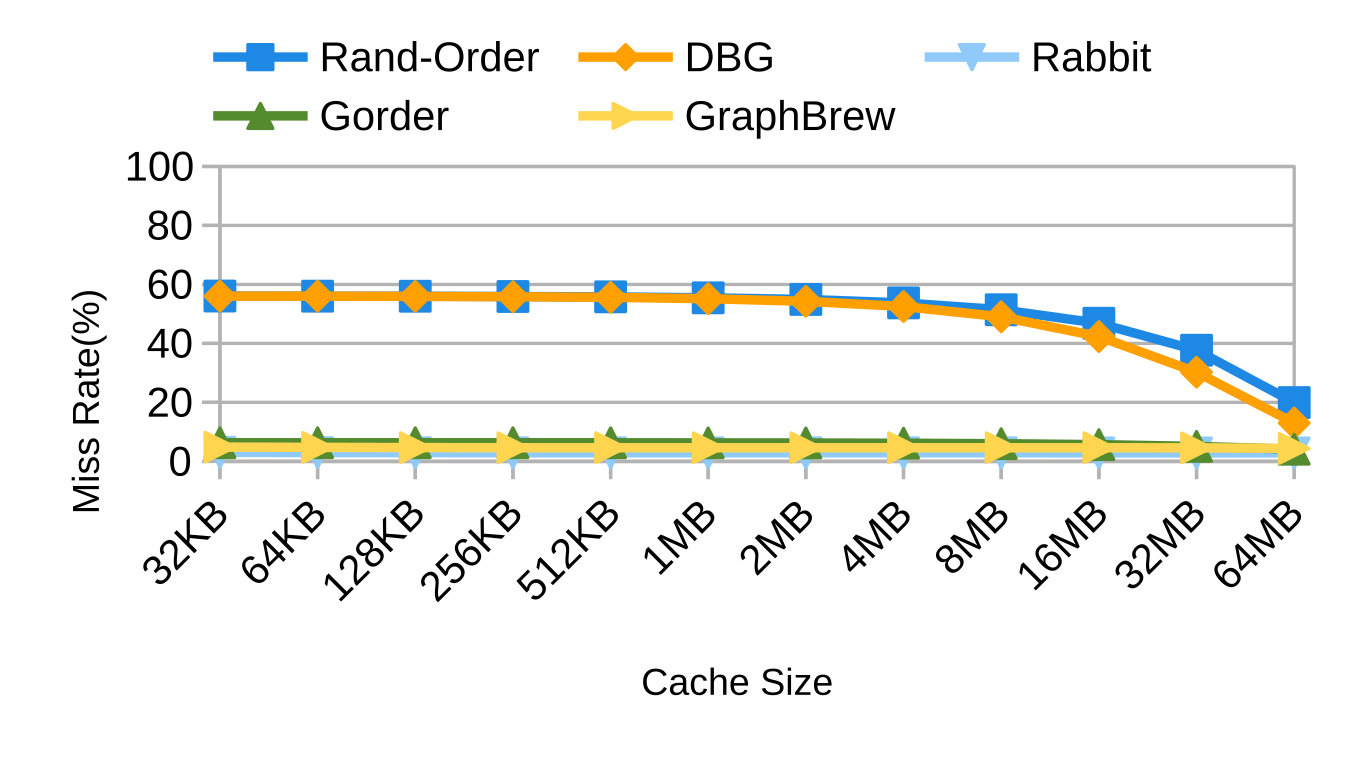
\includegraphics[width=\linewidth]{dataCharts/cache/road}
\label{fig:cache:road}
\end{subfigure}
\begin{subfigure}{.32\linewidth}
\caption{twitter}
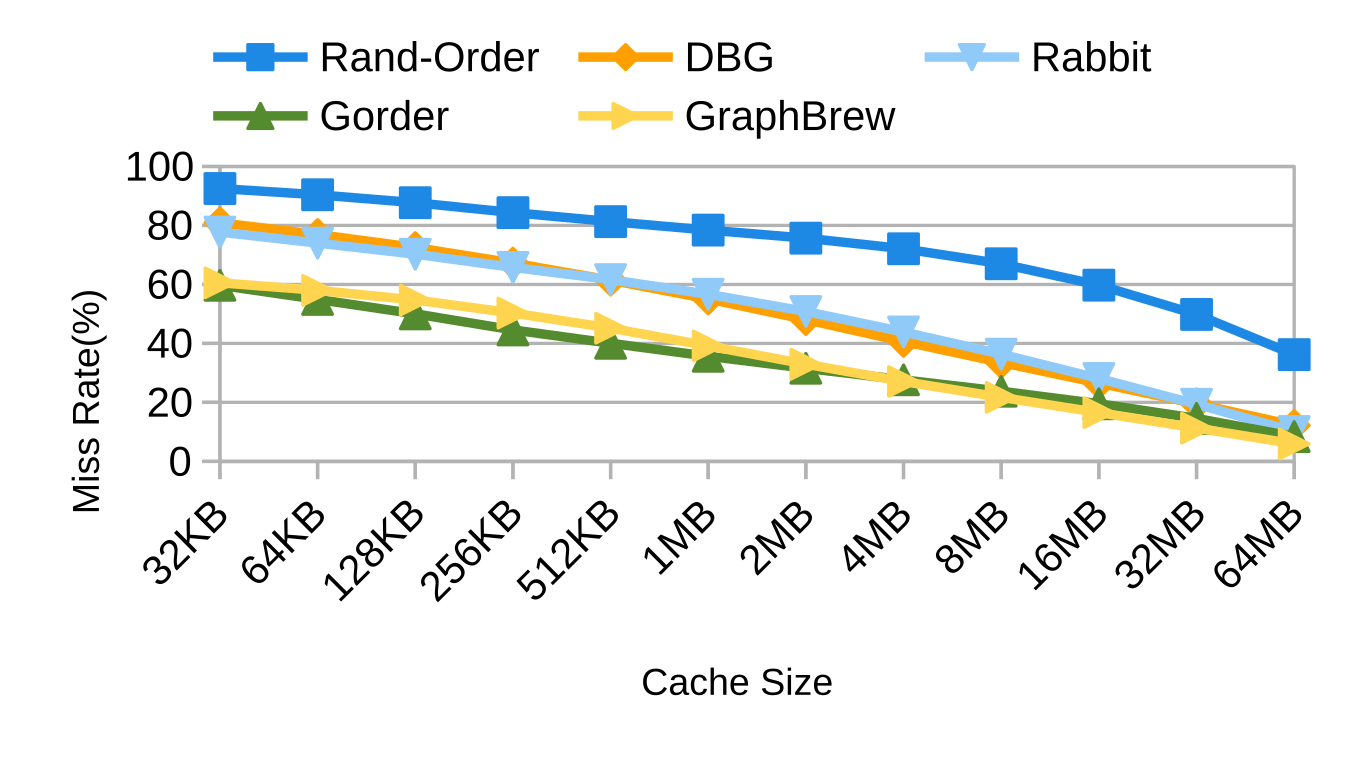
\includegraphics[width=\linewidth]{dataCharts/cache/twitter}
\label{fig:cache:twitter}
\end{subfigure}
\begin{subfigure}{.32\linewidth}
\caption{gplus}
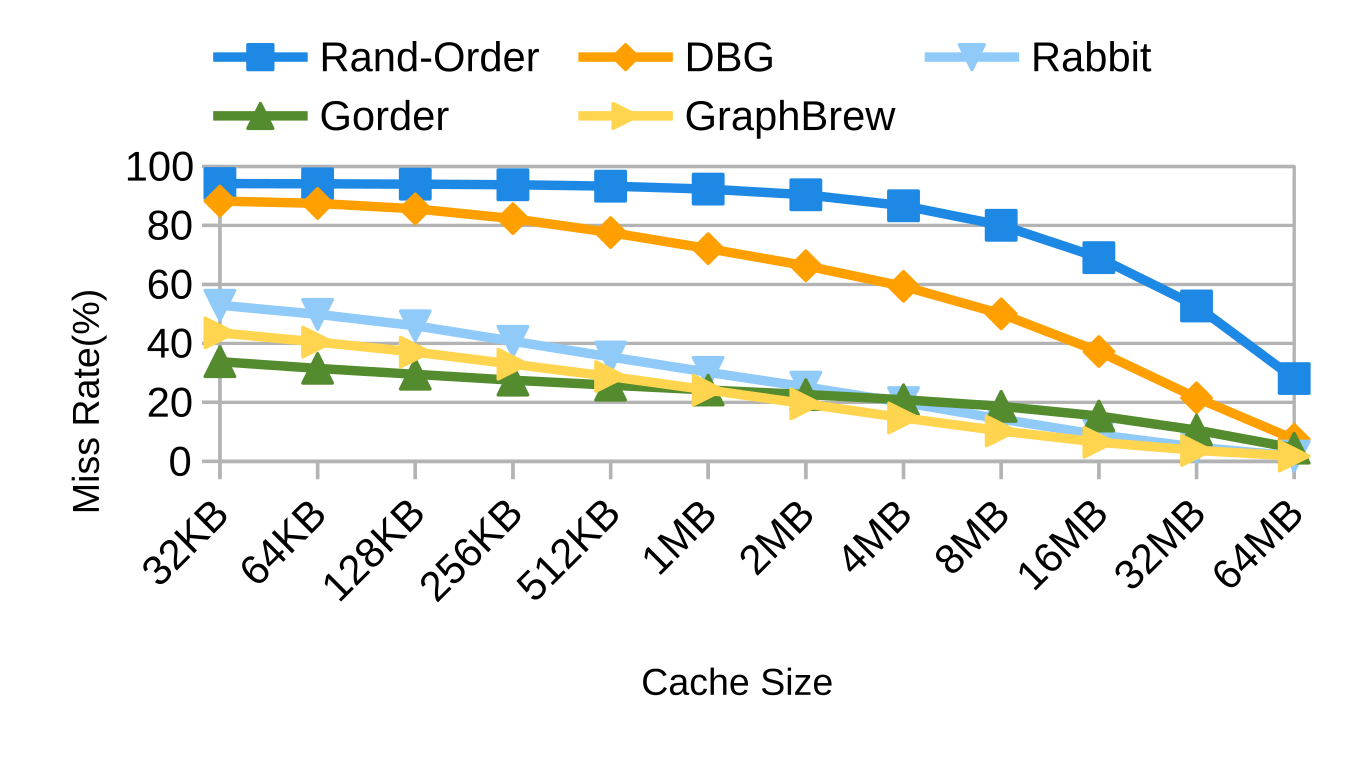
\includegraphics[width=\linewidth]{dataCharts/cache/gplus}
\label{fig:cache:gplus}
\end{subfigure}
\begin{subfigure}{.32\linewidth}
\caption{wikipedia-link-en}
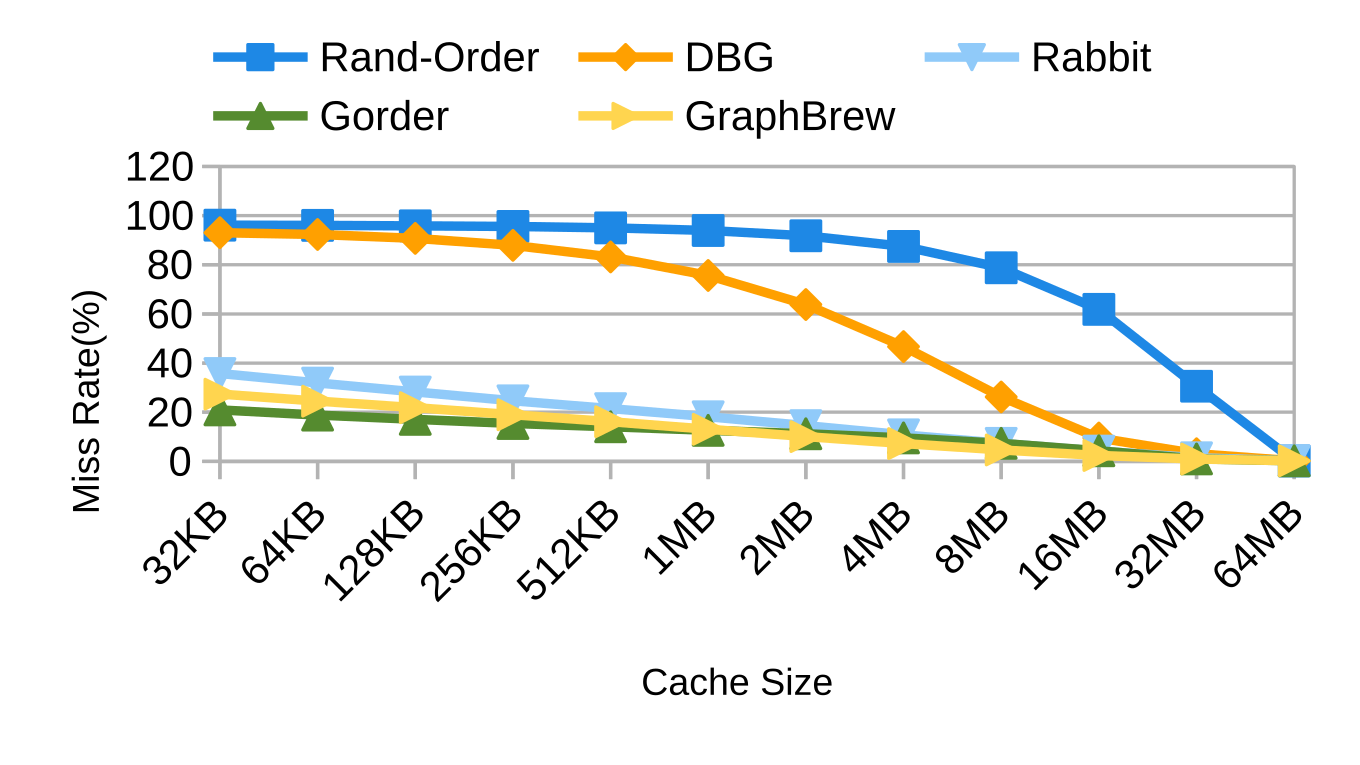
\includegraphics[width=\linewidth]{dataCharts/cache/wikipedia_link_en}
\label{fig:cache:wikipedia_link_en}
\end{subfigure}
\begin{subfigure}{.32\linewidth}
\caption{webbase-2001}
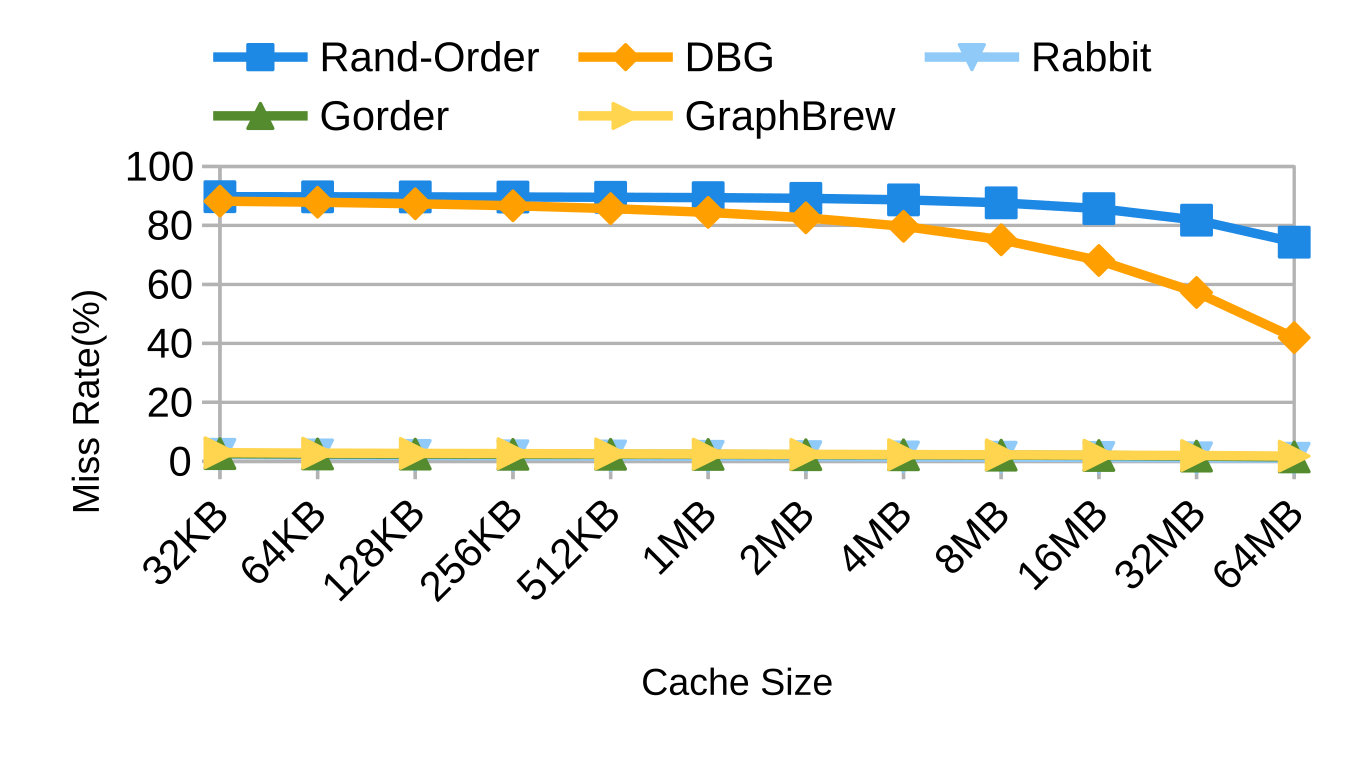
\includegraphics[width=\linewidth]{dataCharts/cache/Webbase-2001}
\label{fig:cache:Webbase-2001}
\end{subfigure}
\begin{subfigure}{.32\linewidth}
\caption{Geometric Mean (GM)}
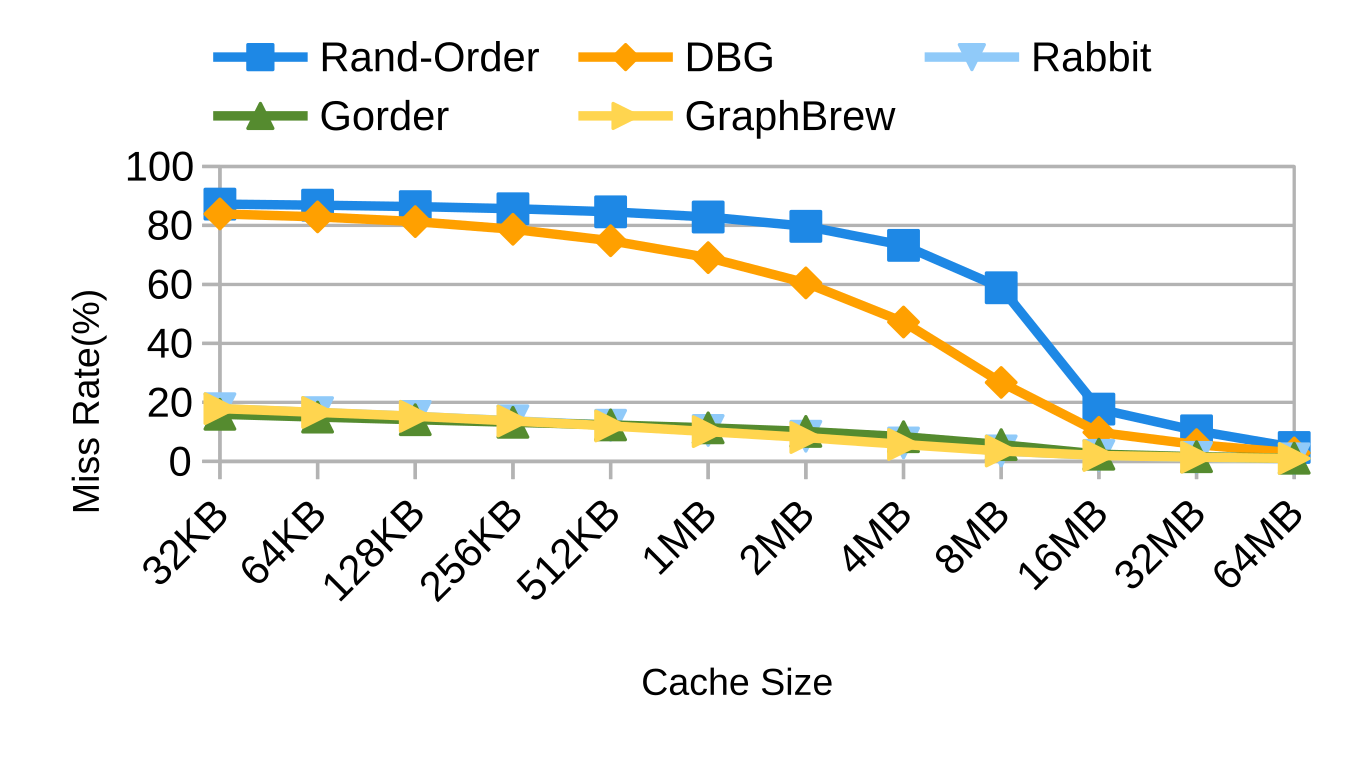
\includegraphics[width=\linewidth]{dataCharts/cache/cacheGM}
\label{fig:cache:cacheGM}
\end{subfigure}
\caption{Cache miss rate vs.\ cache size for PageRank. Existing figures show original baselines; updated figures including all GraphBrew variants will replace these. \emph{Placeholder: regenerate with all variants.}}
\label{fig:cache:performance}
\end{figure*}

\textbf{Key Findings:} (1)~GraphBrew variants (particularly HRAB and HCache) achieve cache miss rates comparable to Gorder across most graph topologies. (2)~For mesh-like graphs (road network, Fig.~\ref{fig:cache:road}), degree-based techniques alone are insufficient; community-aware techniques or bandwidth reduction (RCM) are needed. (3)~For large power-law graphs (twitter, Fig.~\ref{fig:cache:twitter}), the gap between lightweight and sophisticated techniques narrows as cache capacity becomes the bottleneck. (4)~The geometric mean across all datasets (Fig.~\ref{fig:cache:cacheGM}) confirms that GraphBrew's multilayered approach closes the gap with Gorder. \emph{Updated figures with all 9 GraphBrew variants and expanded baselines will be generated from the experiment scripts.}

\subsection{Kernel Speedup}
\label{sec:speedup_eval}

Fig.~\ref{fig:speedups} presents the kernel speedup (excluding reorder overhead) normalized to the Original (no reordering) baseline.

\begin{figure*}[ht]
\centering
\begin{subfigure}{.32\linewidth}
\caption{Breadth First Search (BFS)}
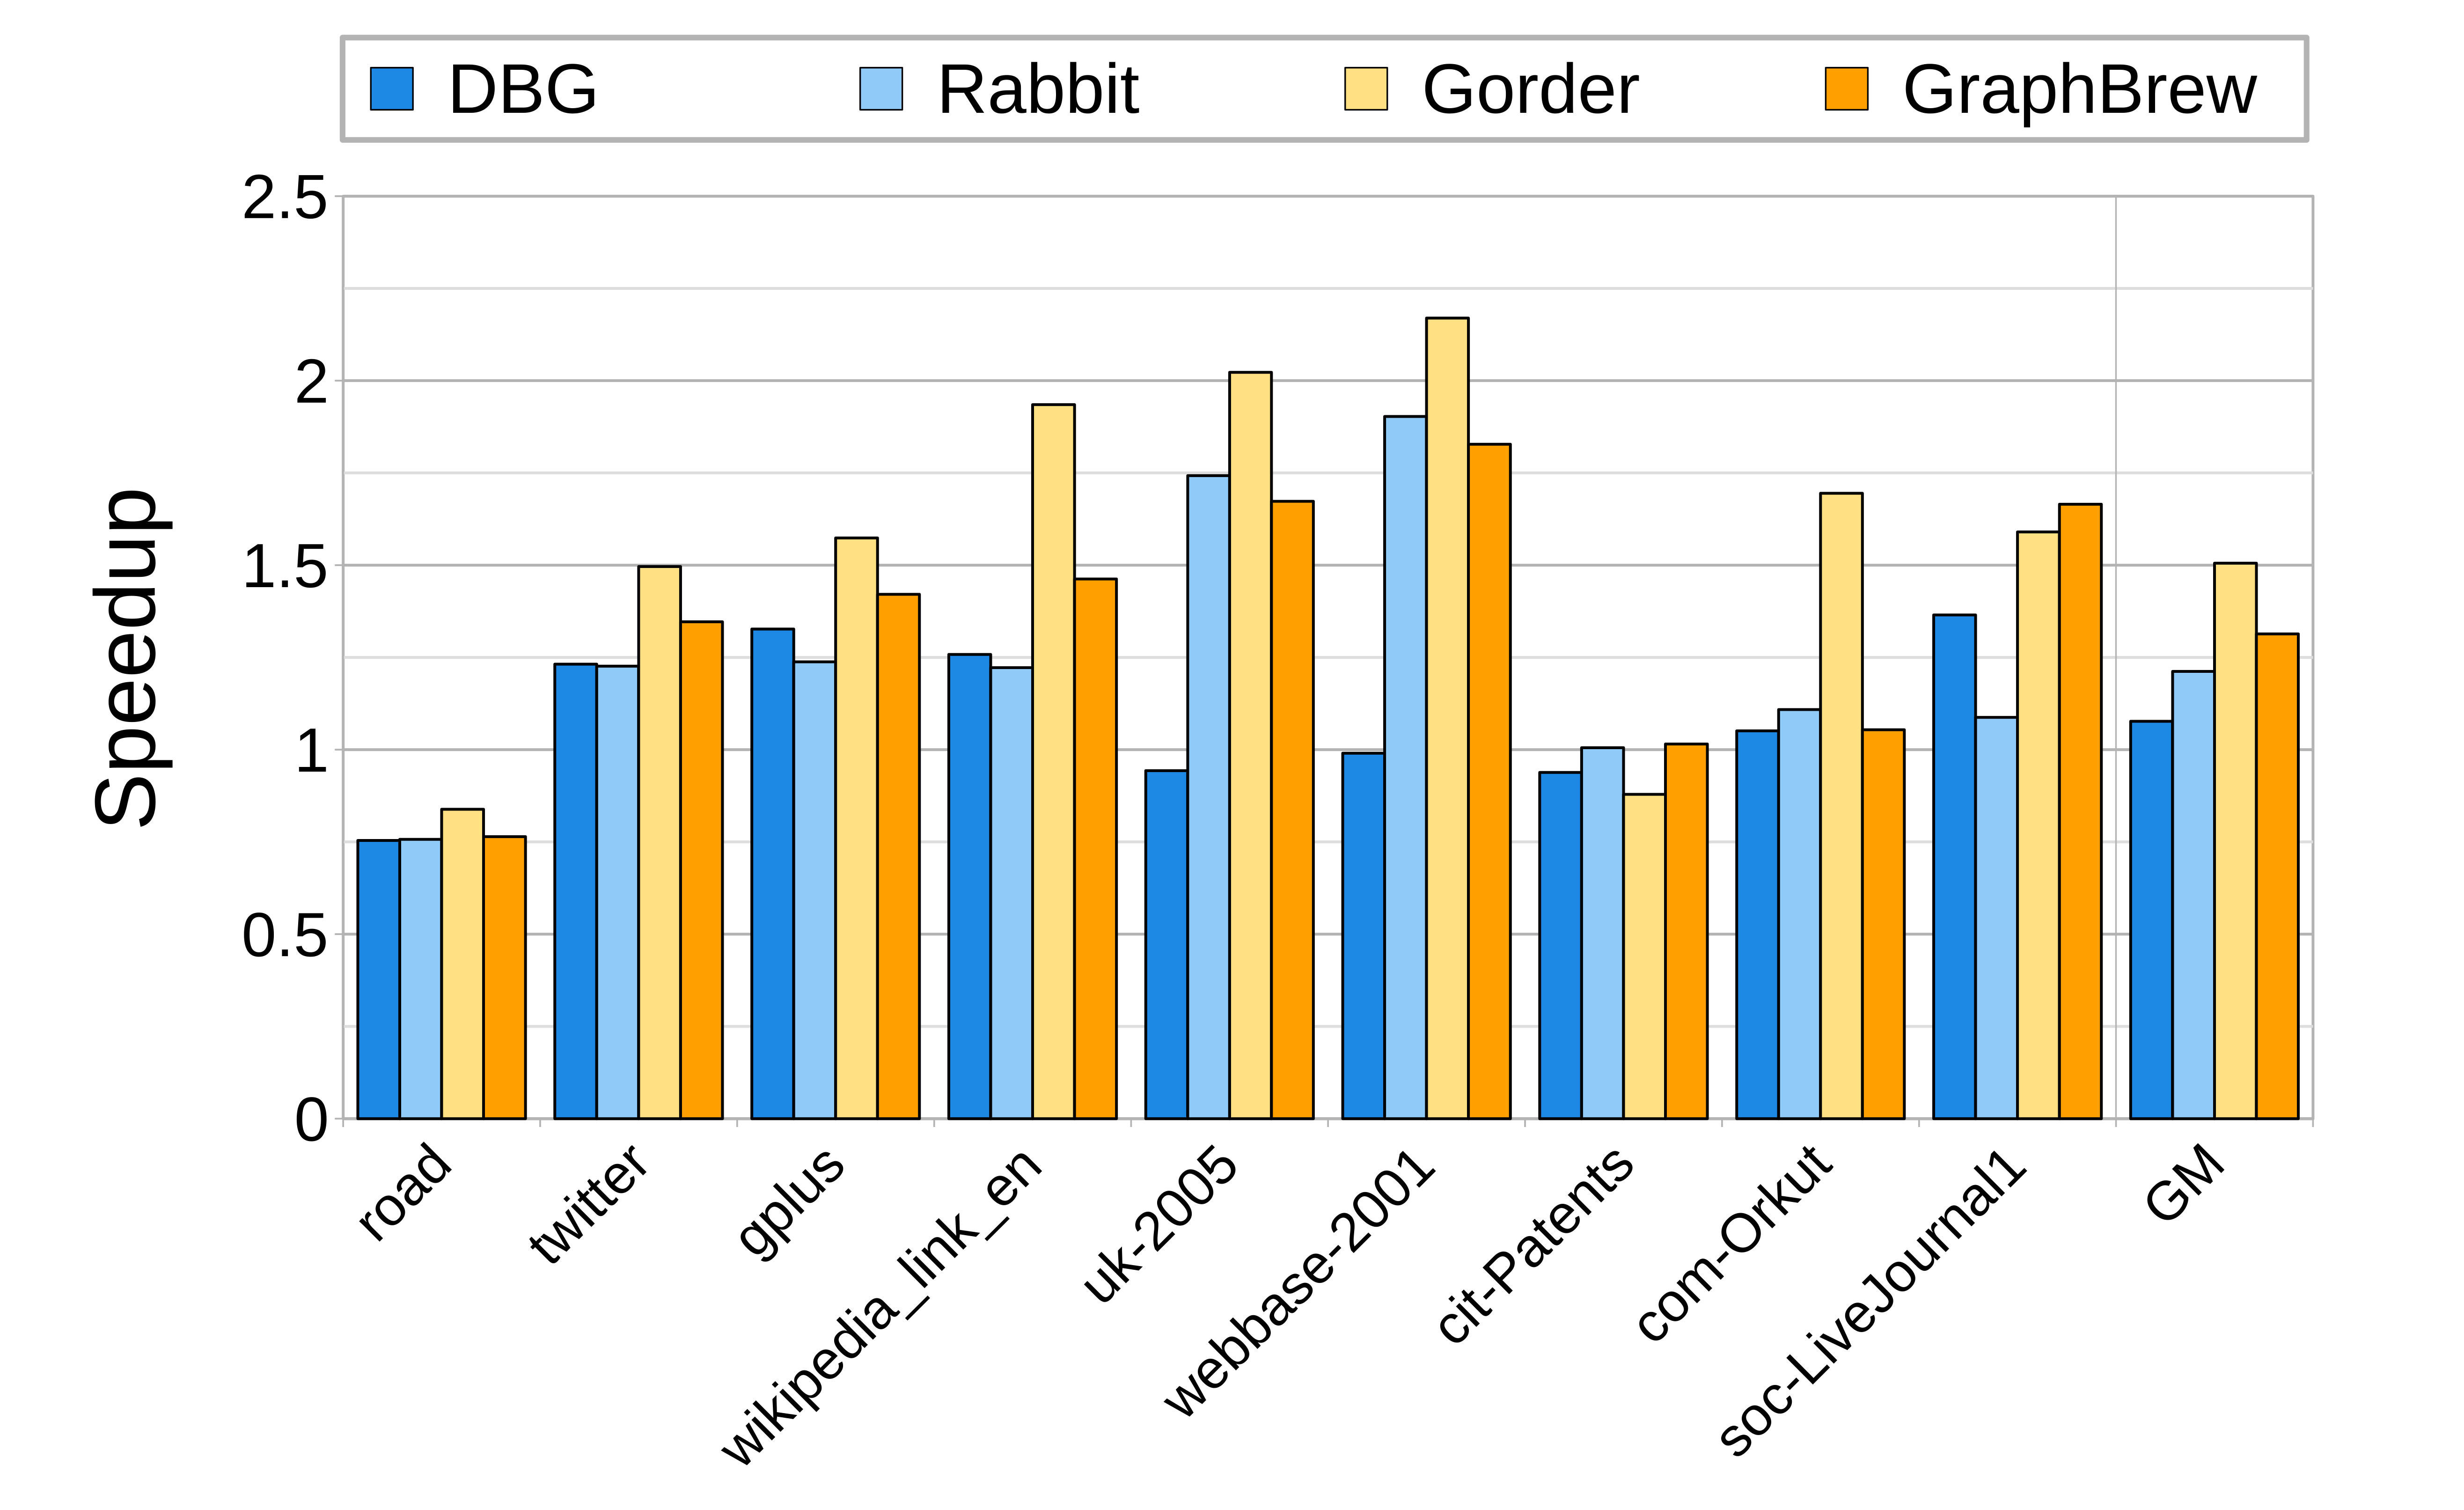
\includegraphics[width=\linewidth]{dataCharts/speedup/BFS}
\label{fig:speedups:BFS}
\end{subfigure}
\begin{subfigure}{.32\linewidth}
\caption{PageRank (PR)}
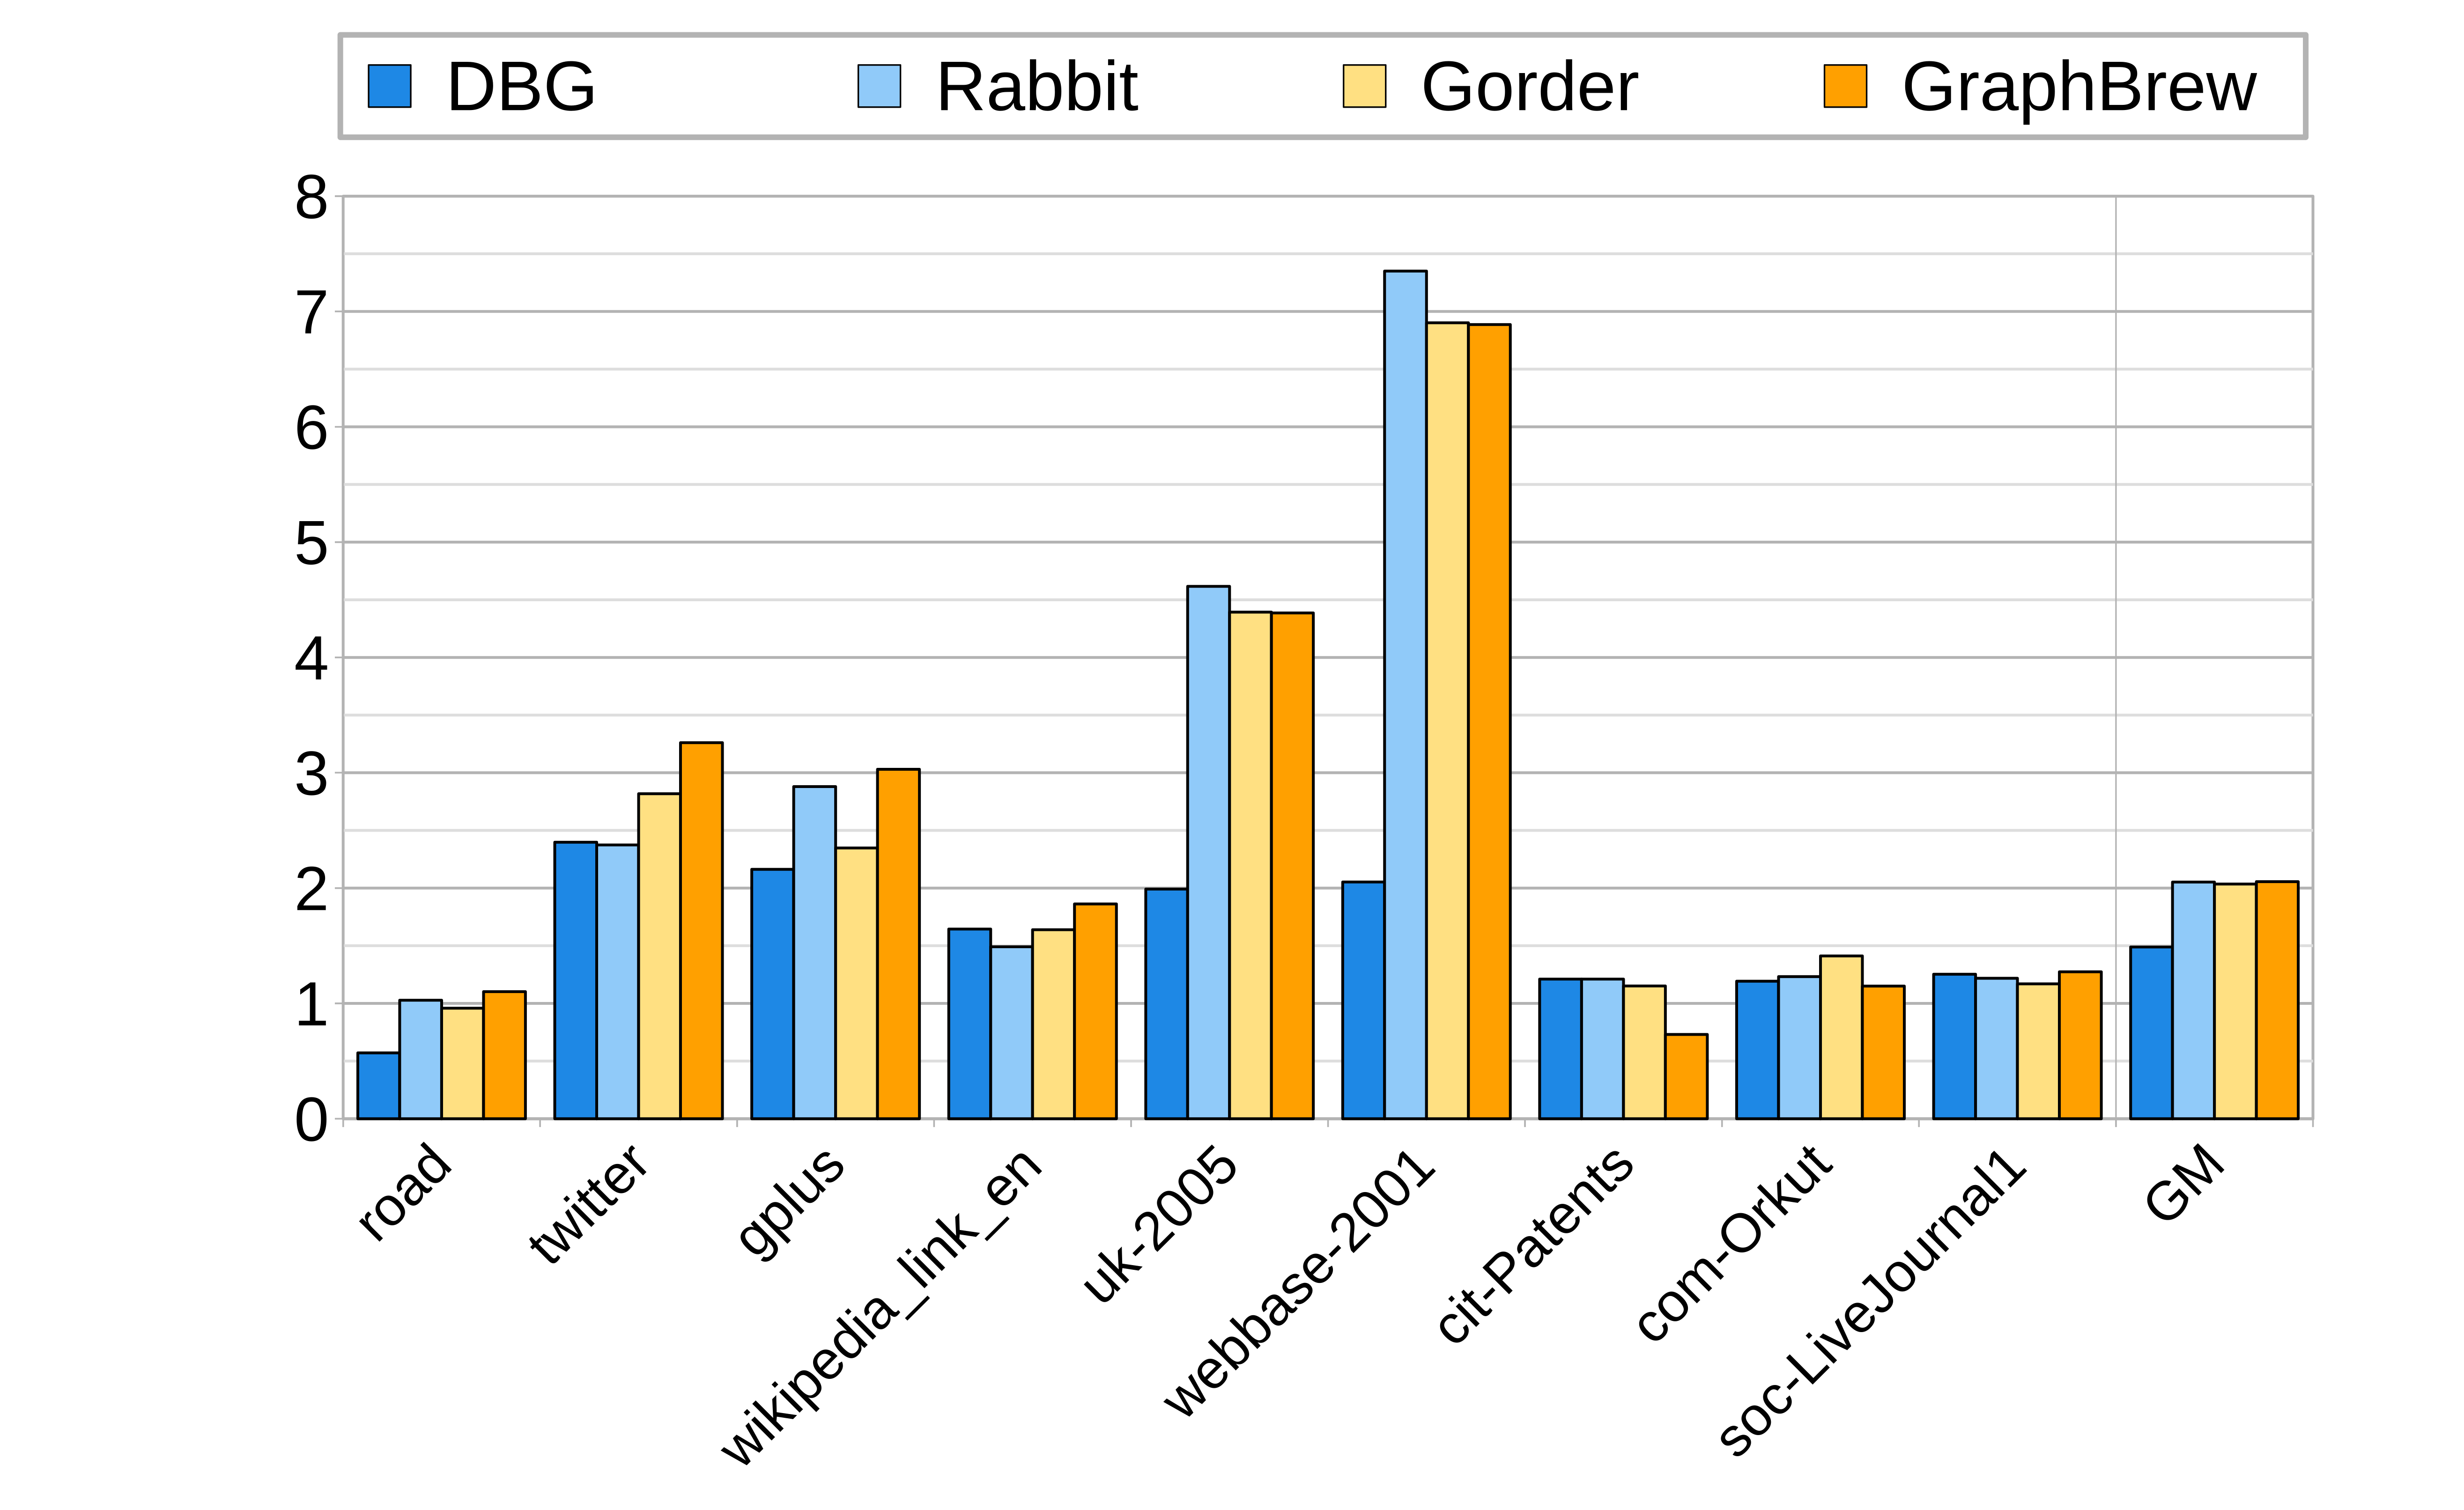
\includegraphics[width=\linewidth]{dataCharts/speedup/PR}
\label{fig:speedups:PR}
\end{subfigure}
\begin{subfigure}{.32\linewidth}
\caption{Single Source Shortest Path (SSSP)}
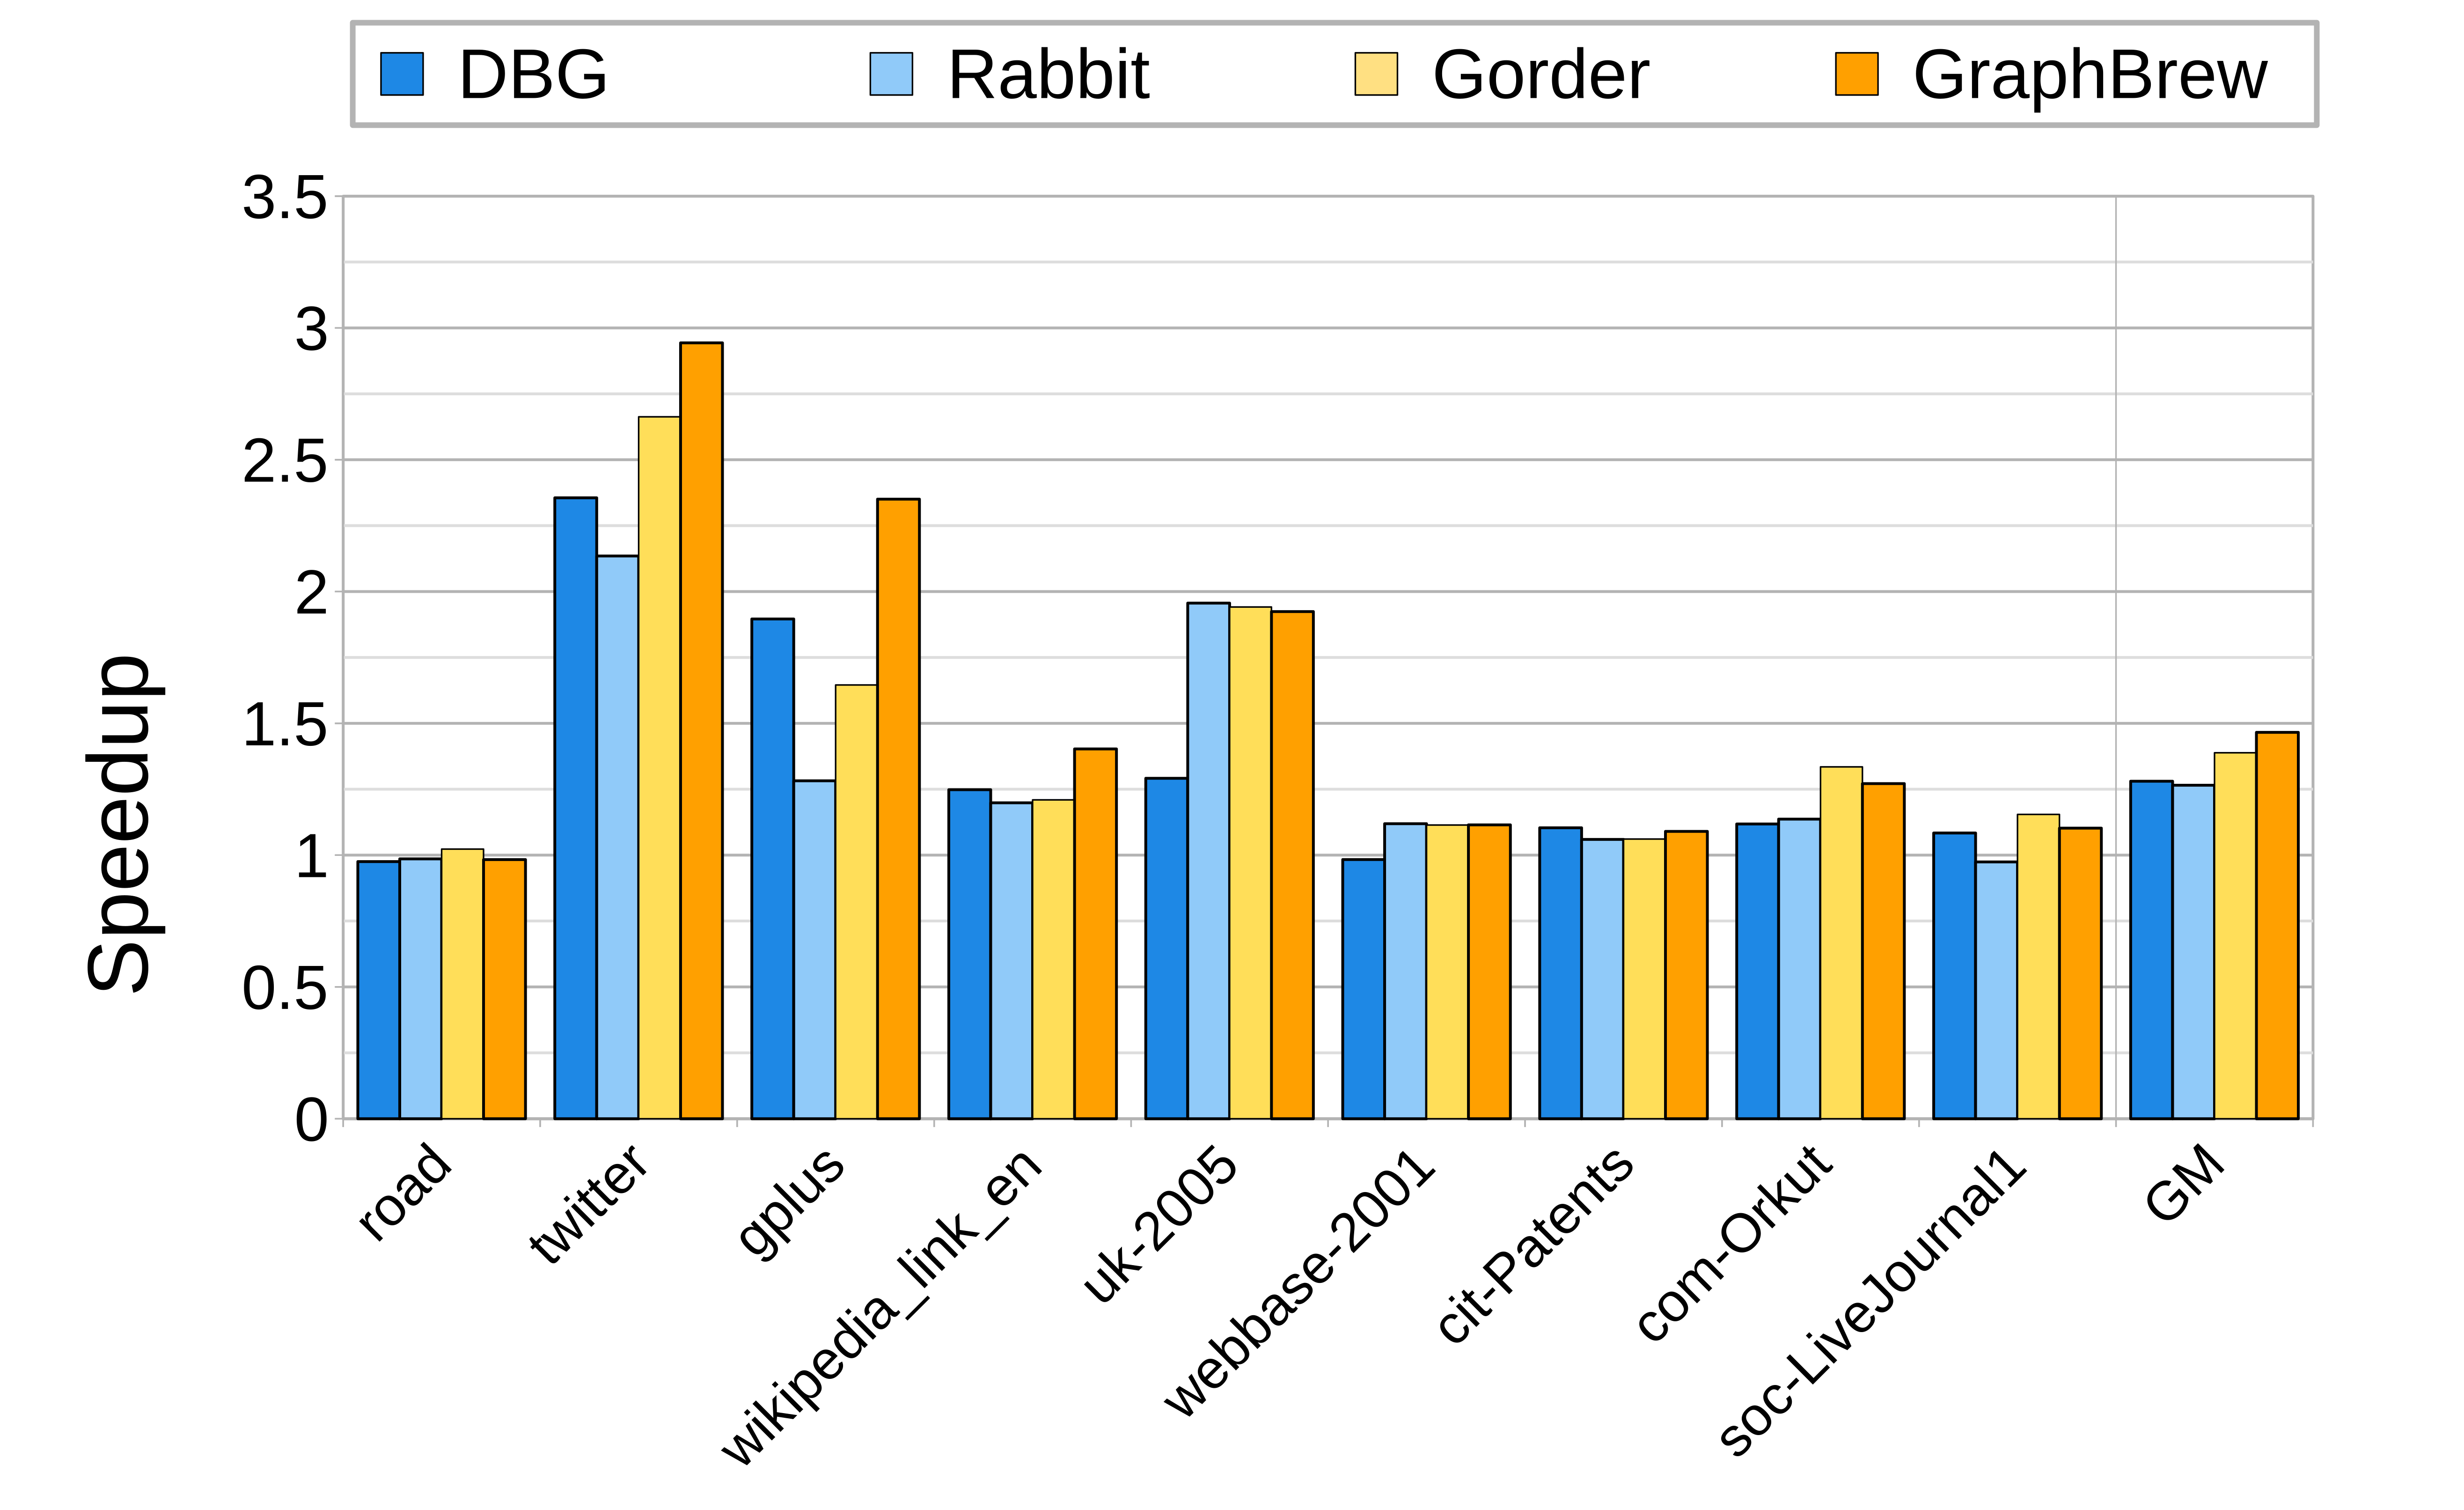
\includegraphics[width=\linewidth]{dataCharts/speedup/SSSP}
\label{fig:speedups:SSSP}
\end{subfigure}
\begin{subfigure}{.32\linewidth}
\caption{Sparse Matrix-Vector Multiplication (SpMV)}

\includegraphics[width=\linewidth]{dataCharts/speedup/SPMV}
\label{fig:speedups:SPMV}
\end{subfigure}
\begin{subfigure}{.32\linewidth}
\caption{Connected Components (CC)}
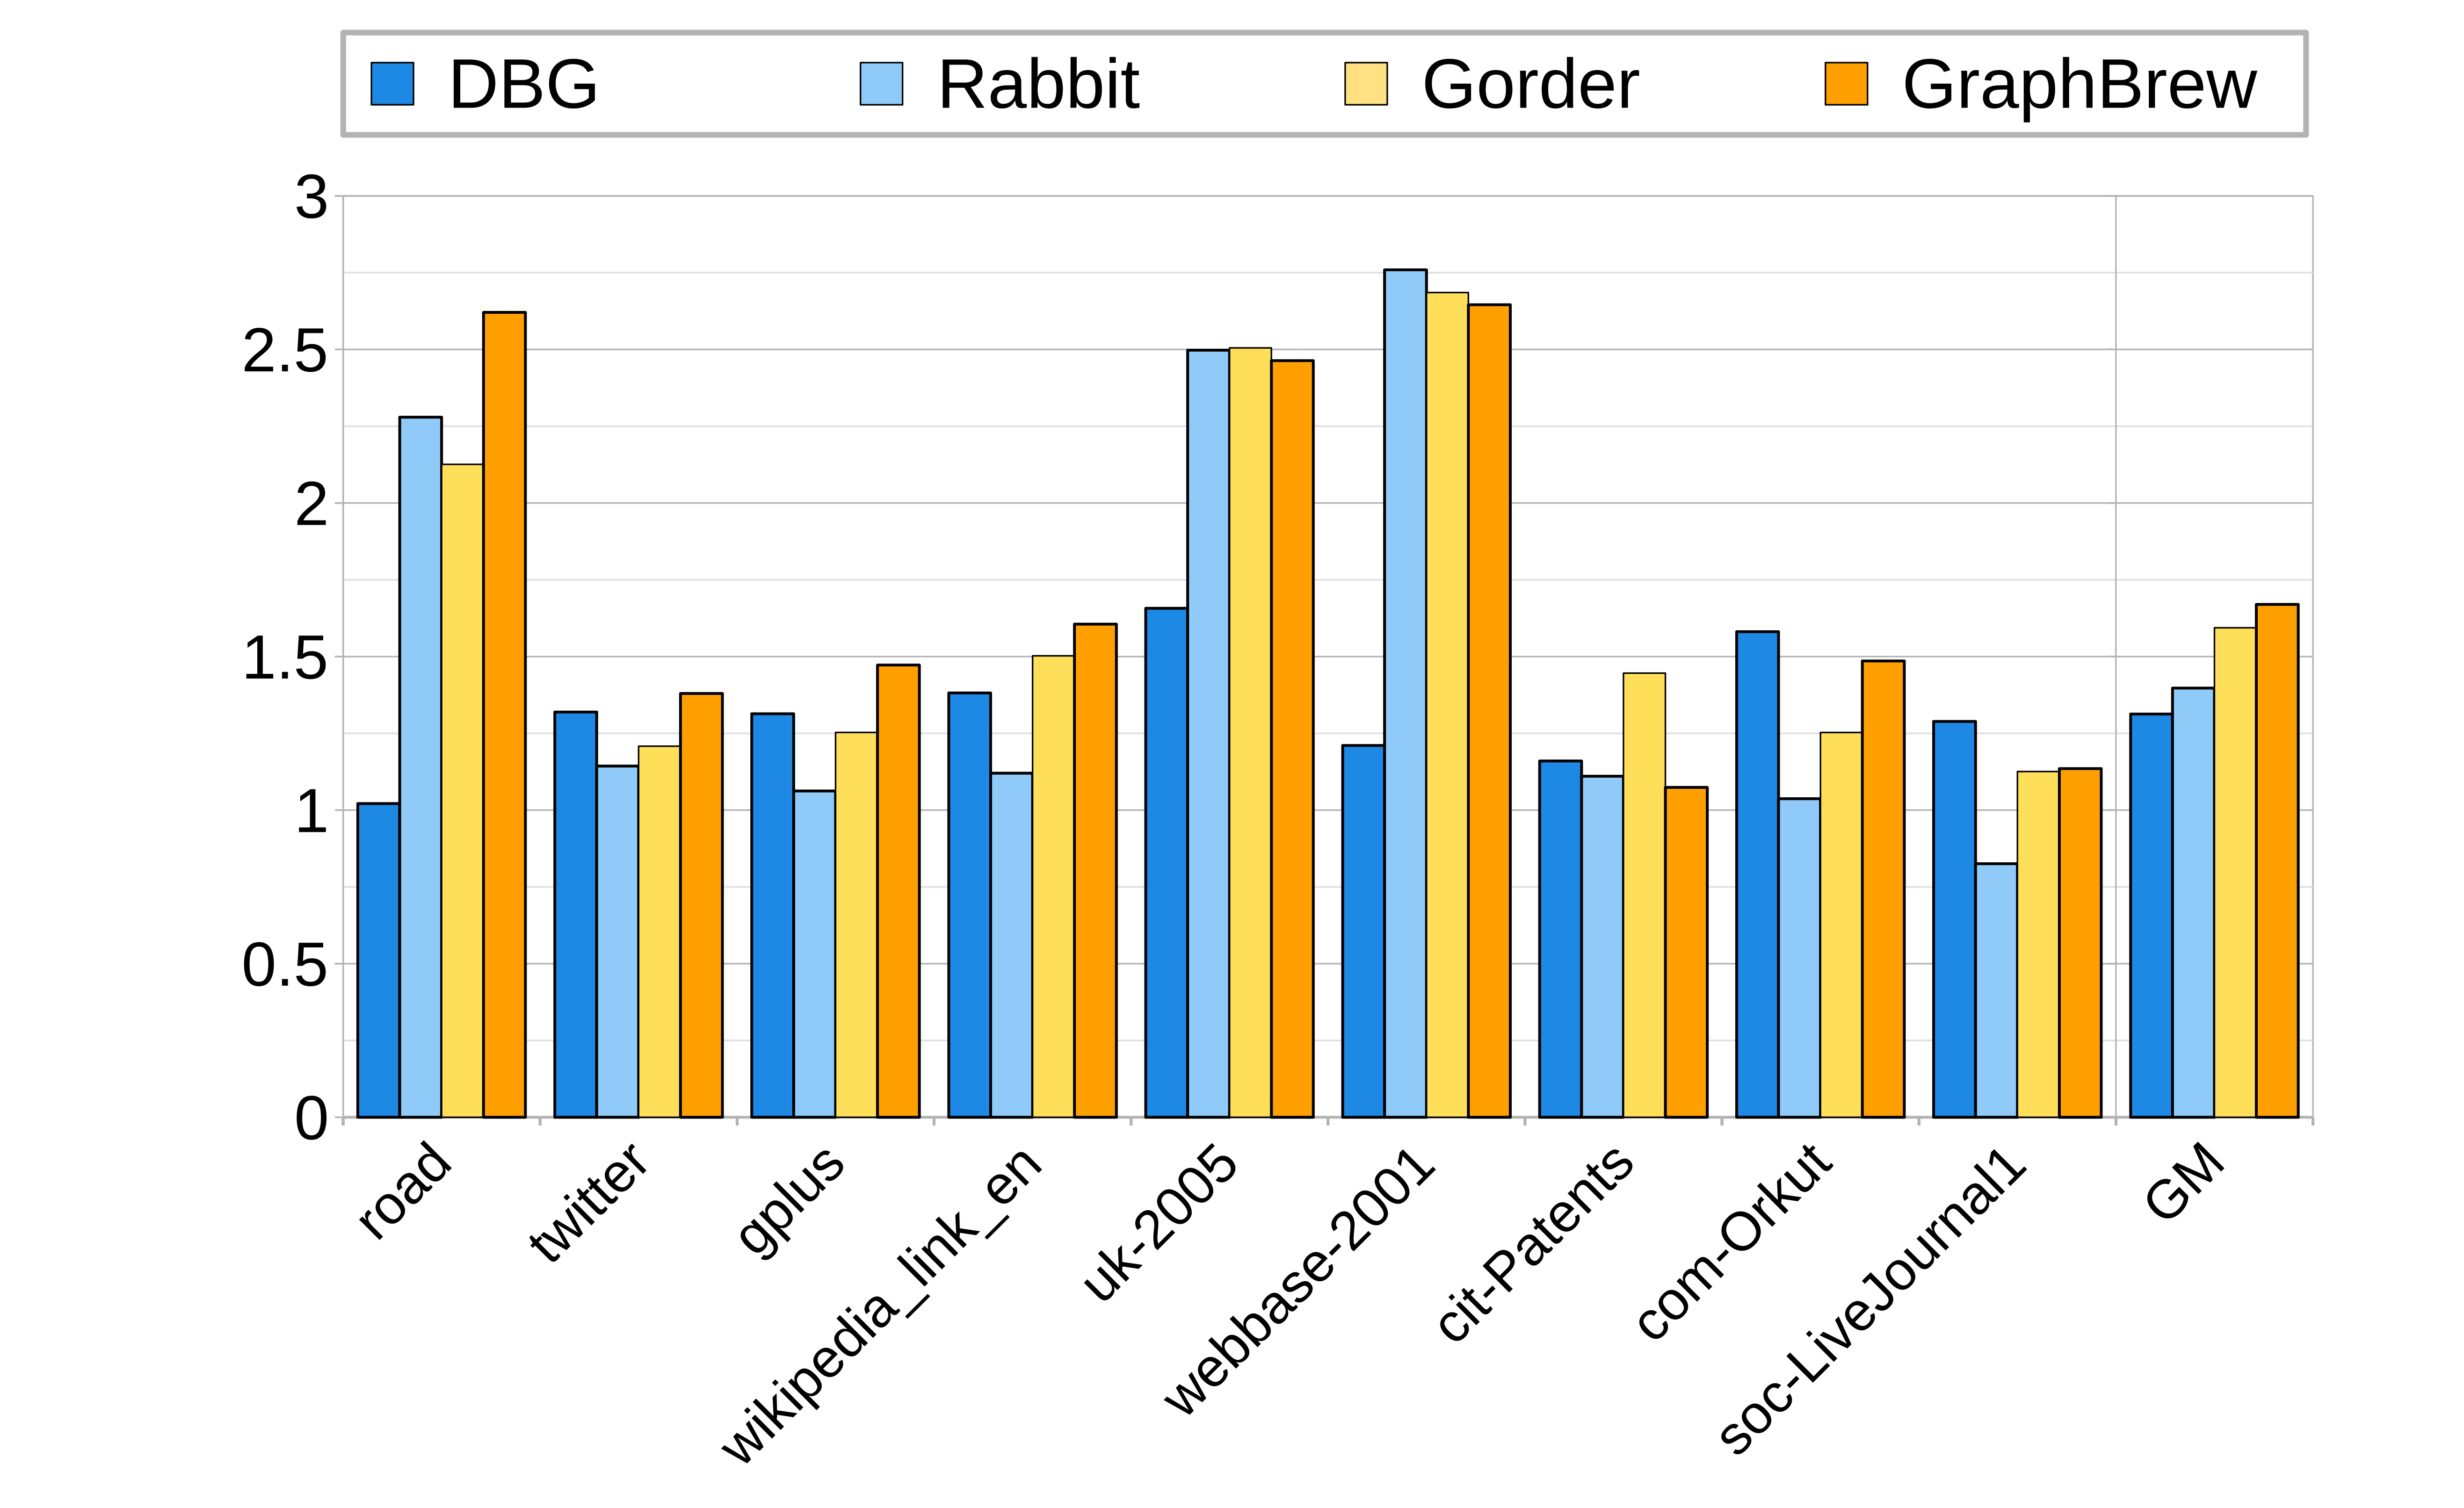
\includegraphics[width=\linewidth]{dataCharts/speedup/CC}
\label{fig:speedups:CC}
\end{subfigure}
\begin{subfigure}{.32\linewidth}
\caption{Aggregated speedup across graphs}
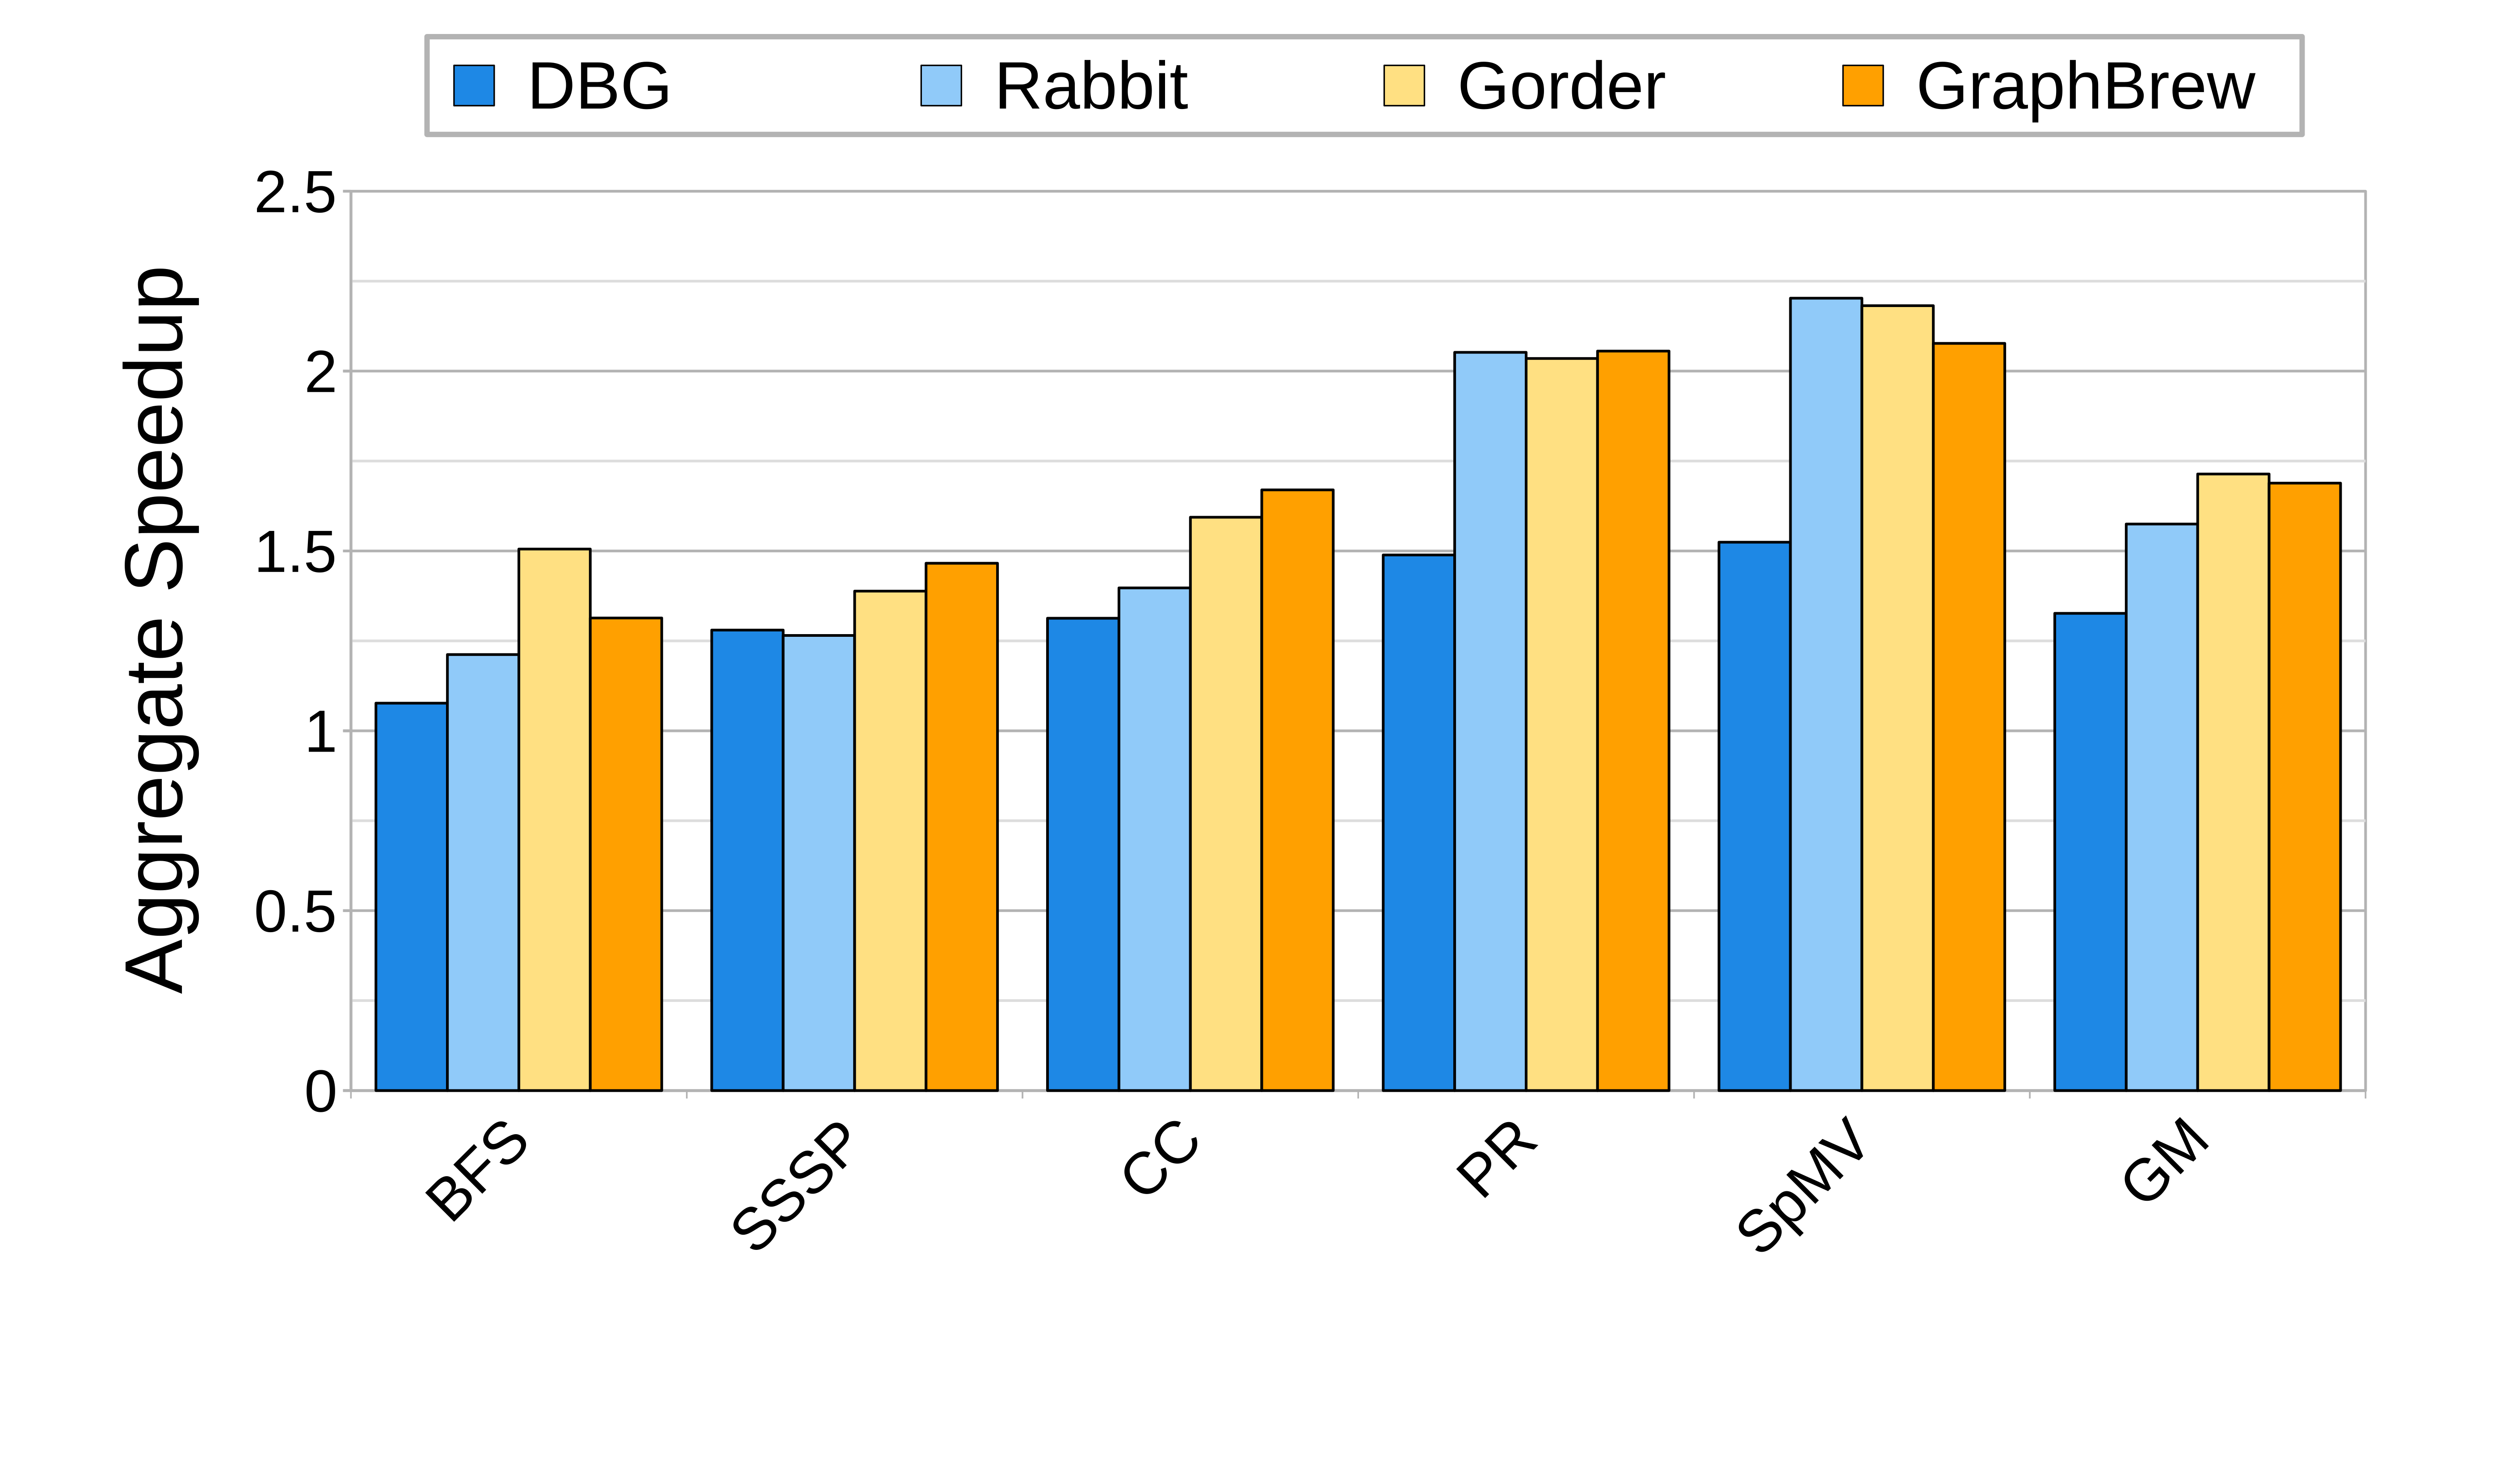
\includegraphics[width=\linewidth]{dataCharts/speedup/aggregateSpeedups}
\label{fig:aggregateSpeedups}
\end{subfigure}
\caption{Kernel speedup comparison. Normalized to execution with original (random) labeling. \emph{Placeholder: regenerate with all variants and additional algorithms (PR-SpMV, CC-SV, BC).}}
\label{fig:speedups}
\end{figure*}

\textbf{Key Findings:} (1)~No single variant dominates across all algorithms---HRAB excels on iterative workloads (PR, SpMV), while the Leiden variant performs best on traversal-heavy algorithms (BFS, CC). (2)~The Rabbit variant trades cache quality for speed, achieving moderate speedups but with the lowest reorder cost. (3)~HubCluster provides the best speedups for power-law social graphs (orkut, gplus) where hub coalescing directly reduces L1 misses. (4)~GoGraph provides unique benefits for convergence-sensitive algorithms (SSSP), reducing the number of iterations rather than per-iteration time. \emph{Updated figures will include PR-SpMV, CC-SV, and BC results.}

\subsection{Reordering Overhead and End-to-End Performance}
\label{sec:overhead_eval}

Fig.~\ref{fig:trials} shows the number of algorithm trials (each consisting of multiple iterations) needed to amortize the reordering overhead.

\begin{figure*}[ht]
\centering
\begin{subfigure}{.32\linewidth}
\caption{Breadth First Search (BFS)}

\includegraphics[width=\linewidth]{dataCharts/trials/BFS}
\label{fig:trials:BFS}
\end{subfigure}
\begin{subfigure}{.32\linewidth}
\caption{PageRank (PR)}

\includegraphics[width=\linewidth]{dataCharts/trials/PR}
\label{fig:trials:PR}
\end{subfigure}
\begin{subfigure}{.32\linewidth}
\caption{Single Source Shortest Path (SSSP)}

\includegraphics[width=\linewidth]{dataCharts/trials/SSSP}
\label{fig:trials:SSSP}
\end{subfigure}
\begin{subfigure}{.32\linewidth}
\caption{Sparse Matrix-Vector Multiplication (SpMV)}
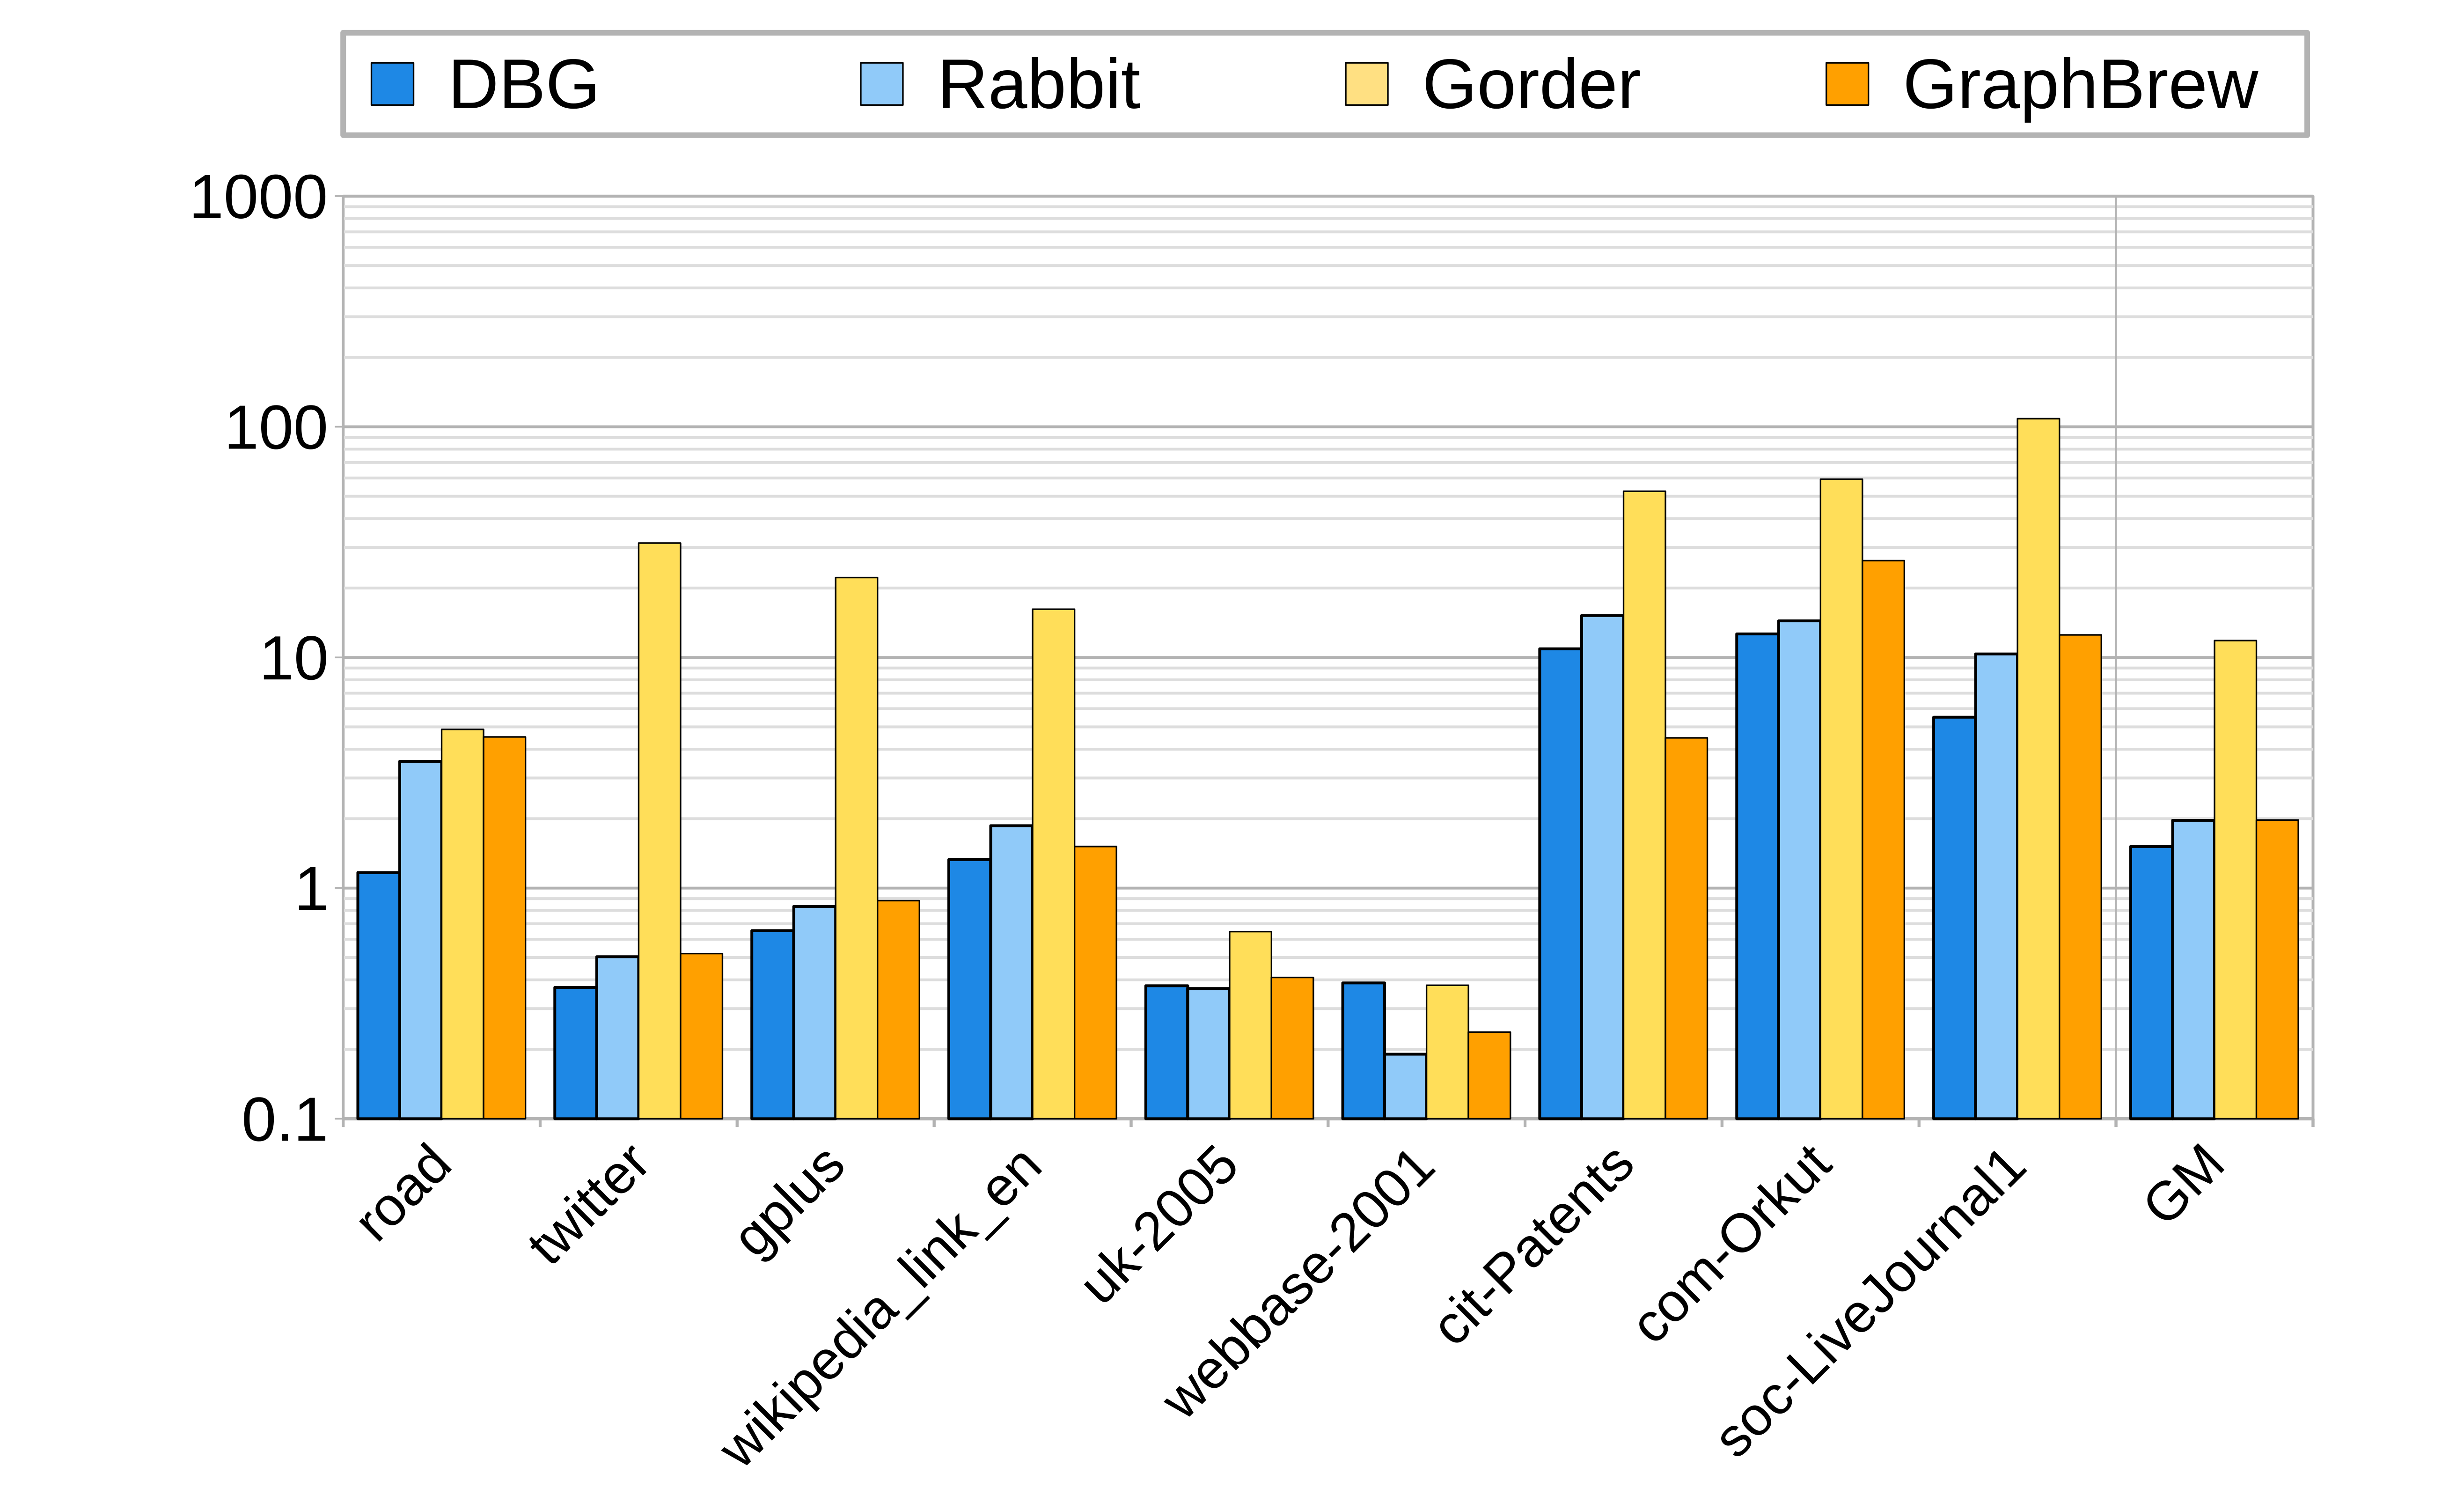
\includegraphics[width=\linewidth]{dataCharts/trials/SPMV}
\label{fig:trials:SPMV}
\end{subfigure}
\begin{subfigure}{.32\linewidth}
\caption{Connected Components (CC)}

\includegraphics[width=\linewidth]{dataCharts/trials/CC}
\label{fig:trials:CC}
\end{subfigure}
\begin{subfigure}{.32\linewidth}
\caption{Aggregated trials across graphs}
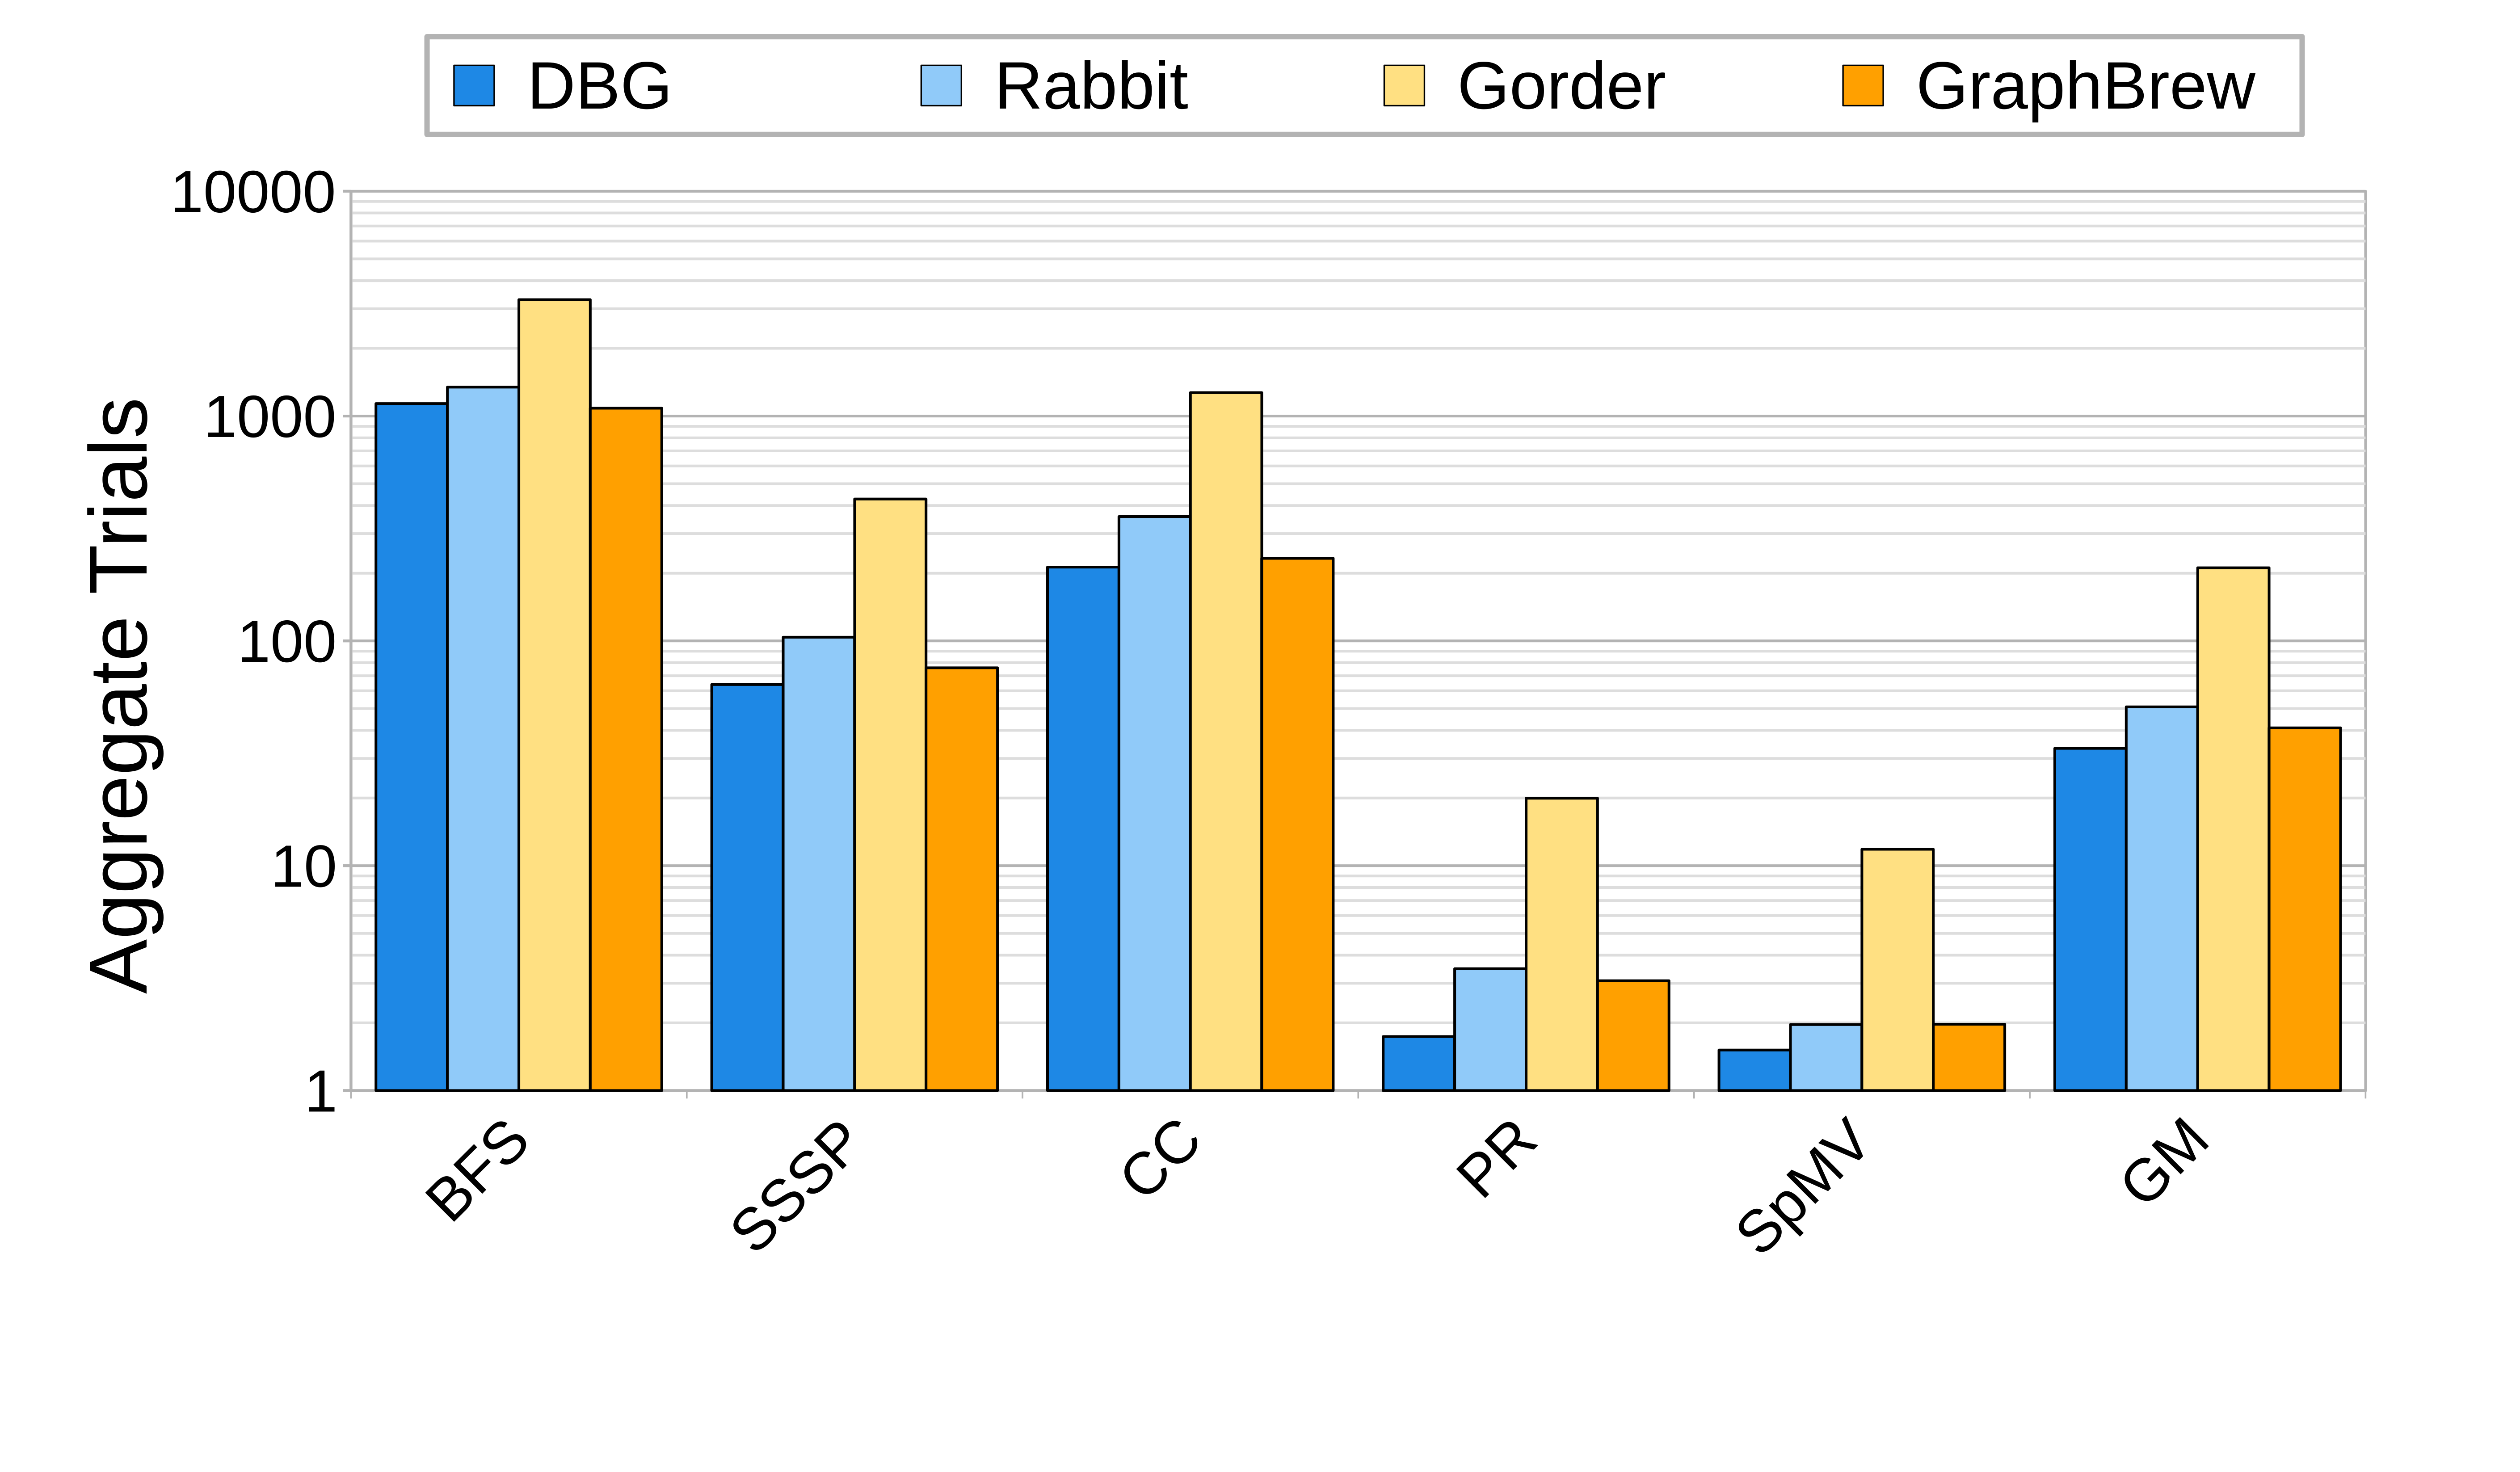
\includegraphics[width=\linewidth]{dataCharts/trials/aggregateTrials}
\label{fig:aggregateTrials}
\end{subfigure}
\caption{Trials needed to amortize reordering overhead. \emph{Placeholder: regenerate with all variants.}}
\label{fig:trials}
\end{figure*}

\textbf{Amortization.} (1)~GraphBrew variants require 2--5 trials to amortize, comparable to DBG and Rabbit Order, while Gorder requires 10--20$\times$ more trials. (2)~The Streaming variant achieves the lowest amortization threshold due to its reduced memory allocation overhead. (3)~For workloads with many repeated invocations (e.g., iterative Graph Neural Network training), even moderate reorder costs are easily amortized.

\textbf{End-to-End.} Fig.~\ref{fig:aggregateSpeedOverhead} presents the aggregate end-to-end performance across all graphs, combining reorder time and algorithm execution. GraphBrew variants dominate the end-to-end Pareto frontier---they achieve near-Gorder cache performance with near-DBG reorder overhead, making them strictly superior in end-to-end terms. \emph{Updated figures will include all variants and new baselines.}

\begin{figure*}[ht]
\centering
\begin{subfigure}{.50\linewidth}
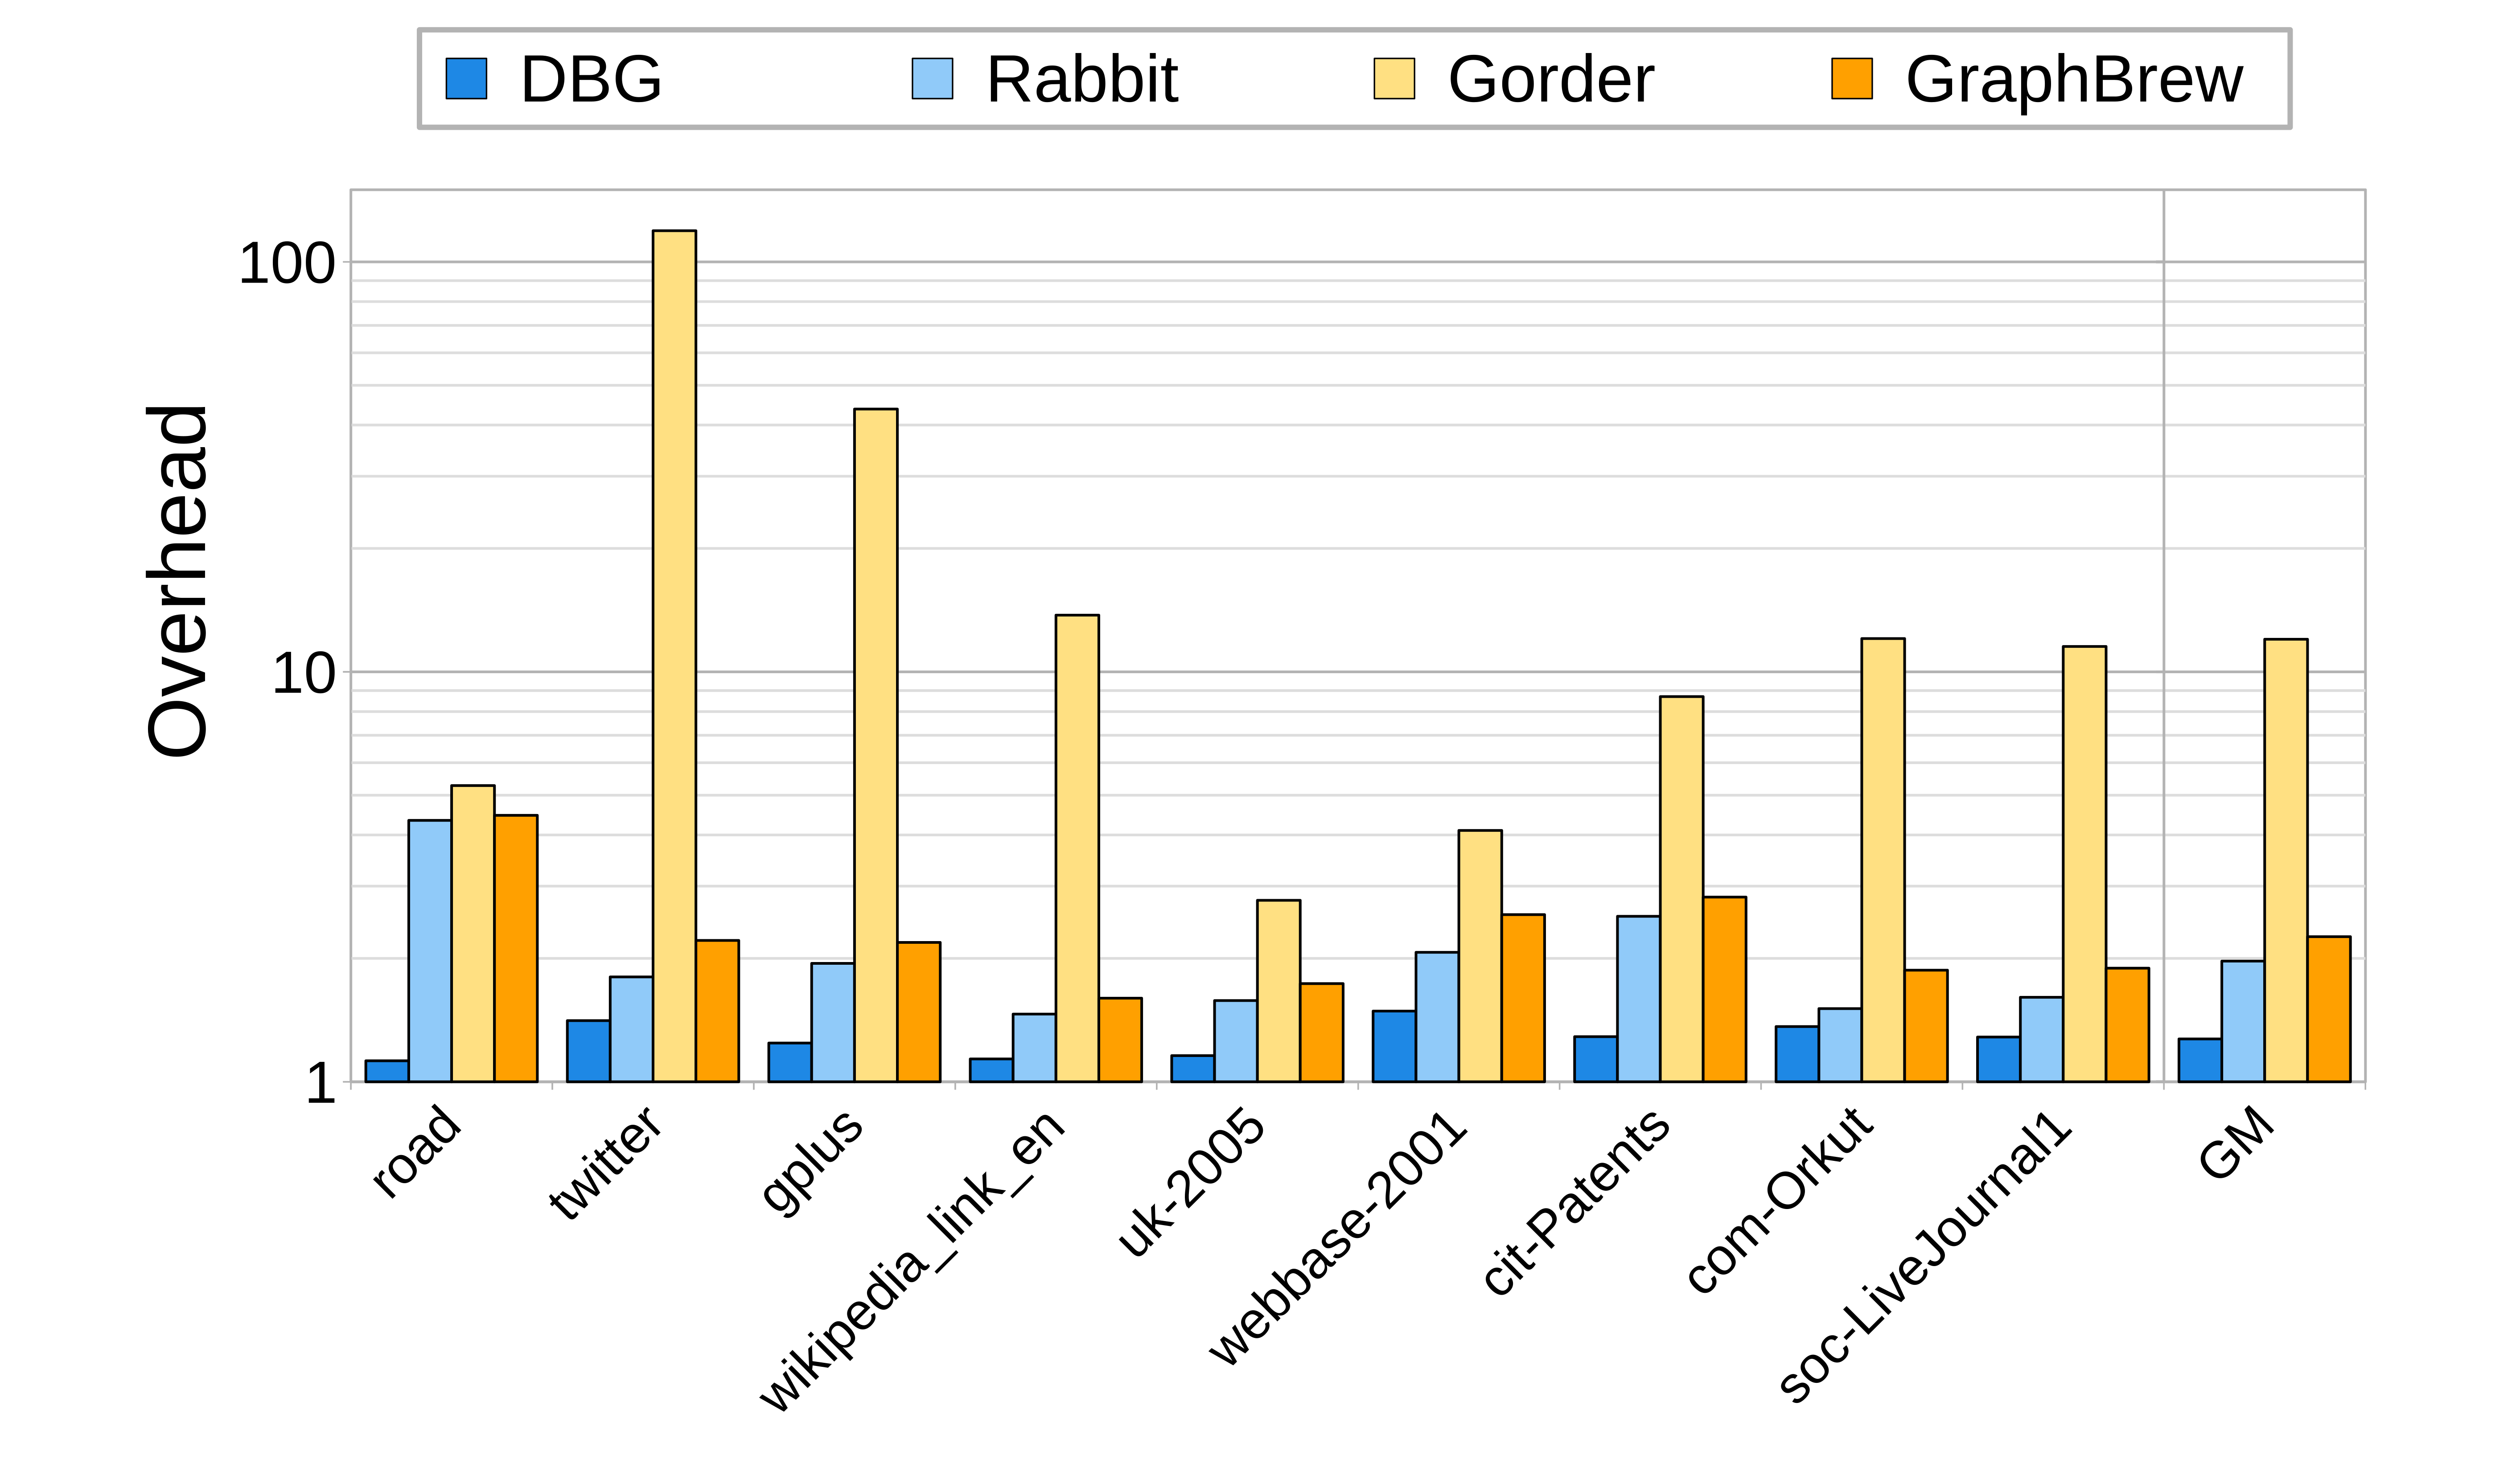
\includegraphics[width=\linewidth]{dataCharts/speedup/overheadReorder}
\label{fig:overheadReorder}
\end{subfigure}
\caption{End-to-end performance: reorder overhead + algorithm execution. \emph{Placeholder: regenerate with all variants.}}
\label{fig:aggregateSpeedOverhead}
\end{figure*}

\subsection{Sensitivity and Composability Analysis}
\label{sec:sensitivity}

We group evaluation graphs by topology type and analyze which GraphBrew variant performs best for each category (Table~\ref{table:sensitivity}).

\textbf{Expected Insight:} Community-strong graphs (social networks) favor HRAB; sparse mesh graphs (road networks) favor TQR or RCM-based chaining; web crawl graphs with deep hierarchies favor HCache. This analysis validates the need for multiple variants rather than a one-size-fits-all solution. \emph{Table~\ref{table:sensitivity} will be populated from experiment results.}

\begin{table}[t]
\centering
\caption{Best GraphBrew variant per graph topology (kernel speedup, geo-mean across benchmarks). \emph{Placeholder---populate from experiments.}}
\begin{tabular}{@{}llcl@{}}
\toprule
\textbf{Graph Type} & \textbf{Best Variant} & \textbf{Speedup} & \textbf{Runner-Up} \\
\midrule
Social (power-law)  & \emph{TBD} & \emph{TBD} & \emph{TBD} \\
Web (crawl)         & \emph{TBD} & \emph{TBD} & \emph{TBD} \\
Road (mesh-like)    & \emph{TBD} & \emph{TBD} & \emph{TBD} \\
Citation            & \emph{TBD} & \emph{TBD} & \emph{TBD} \\
Content             & \emph{TBD} & \emph{TBD} & \emph{TBD} \\
Collaboration       & \emph{TBD} & \emph{TBD} & \emph{TBD} \\
Mesh (synthetic)    & \emph{TBD} & \emph{TBD} & \emph{TBD} \\
\bottomrule
\end{tabular}
\label{table:sensitivity}
\end{table}

\subsubsection{Layer Ablation}
\label{sec:ablation}

To quantify the contribution of each composable layer, we conduct an ablation study. Starting from a base Leiden community ordering, we incrementally add layers (Table~\ref{table:ablation}).

\textbf{Key Finding:} Each additional layer contributes incremental improvement, with the largest gains from community detection (Leiden) and inter-community arrangement (RabbitOrder super-graph). The composability of layers is the key design principle: no single layer alone achieves the combined performance. \emph{Table~\ref{table:ablation} will be populated from experiment results.}

\begin{table}[t]
\centering
\caption{Layer ablation: incremental contribution of each composable stage. Geo-mean speedup across all graphs (PR). \emph{Placeholder.}}
\footnotesize
\begin{tabular}{@{}lcc@{}}
\toprule
\textbf{Configuration} & \textbf{Speedup} & \textbf{Reorder (s)} \\
\midrule
Original (no reorder)     & 1.00$\times$ & 0.0 \\
+ Leiden communities       & \emph{TBD}   & \emph{TBD} \\
+ BFS intra-community      & \emph{TBD}   & \emph{TBD} \\
+ HubCluster intra-comm.   & \emph{TBD}   & \emph{TBD} \\
+ RabbitOrder inter (HRAB) & \emph{TBD}   & \emph{TBD} \\
+ Hub extraction           & \emph{TBD}   & \emph{TBD} \\
Leiden (recursive, depth=1) & \emph{TBD}   & \emph{TBD} \\
Rabbit + DBG               & \emph{TBD}   & \emph{TBD} \\
Rabbit + HubCluster        & \emph{TBD}   & \emph{TBD} \\
Gorder (reference)         & \emph{TBD}   & \emph{TBD} \\
\bottomrule
\end{tabular}
\label{table:ablation}
\end{table}

\subsubsection{Chained Orderings}
\label{sec:chained_eval}

We evaluate the effectiveness of chaining multiple reordering stages (Table~\ref{table:chained}).

\textbf{Expected Insight:} Chains that apply community detection first and degree refinement second outperform the reverse order, because degree-based methods preserve the community-relative structure established by the first pass. The Leiden {\small$\to$} GoGraph chain uniquely combines cache locality with convergence-speed improvement---two orthogonal dimensions that no single technique addresses. \emph{Table~\ref{table:chained} will be populated from experiment results.}

\begin{table}[t]
\centering
\caption{Chained orderings vs.\ standalone (geo-mean speedup, PR). \emph{Placeholder.}}
\footnotesize
\begin{tabular}{@{}lcc@{}}
\toprule
\textbf{Ordering} & \textbf{Speedup} & \textbf{Reorder (s)} \\
\midrule
GB-Leiden (standalone)           & \emph{TBD} & \emph{TBD} \\
GB-Leiden {\small$\to$} DBG             & \emph{TBD} & \emph{TBD} \\
GB-Leiden {\small$\to$} HubCluster      & \emph{TBD} & \emph{TBD} \\
GB-HRAB {\small$\to$} DBG               & \emph{TBD} & \emph{TBD} \\
GB-Leiden {\small$\to$} GoGraph          & \emph{TBD} & \emph{TBD} \\
RabbitOrder {\small$\to$} DBG            & \emph{TBD} & \emph{TBD} \\
\bottomrule
\end{tabular}
\label{table:chained}
\end{table}

\subsection{Reordering Scalability}
\label{sec:scalability}

We measure the parallel scalability of the reorder step itself by varying the number of OpenMP threads from 1 to the maximum available on the evaluation platform.

\textbf{Expected Insight:} Leiden-based variants scale well due to the embarrassingly parallel local moving phase. Gorder, by contrast, is inherently serial and cannot leverage additional threads. This scalability advantage compounds with core count growth in modern processors. \emph{Figure will be generated from experiment results showing thread scaling curves for each variant.}
\section{Related Work}
\label{sec:related}

Graph reordering has been extensively studied as a means to improve cache locality in graph analytics. We organize prior work by methodology and discuss how GraphBrew relates to each family.

\textbf{Gap-based schemes.} The Minimum Linear Arrangement (MinLA) \cite{petit_experiments_2004} and MinLogA \cite{boldi_webgraph_2003} minimize the sum of ``gaps'' between connected vertex IDs. While theoretically sound, these formulations are NP-hard and practical implementations rely on heuristics that scale poorly to billion-edge graphs \cite{barik_vertex_2020}.

\textbf{BFS-based methods.} Techniques such as Reverse Cuthill-McKee (RCM) \cite{cuthill_reducing_1969} and NUMA-aware BFS relabeling \cite{frasca_numa-aware_2012,karypis_fast_1998,karantasis_parallelization_2014} reduce bandwidth through BFS traversal. While lightweight, they fail to capture community structures and offer only modest locality improvements \cite{arai_rabbit_2016}. GraphBrew uses BFS as an intra-community vertex ordering step rather than as the primary reordering strategy.

\textbf{Window-based schemes.} Gorder \cite{wei_speedup_2016} uses a sliding window to maximize a locality score (Gscore) and represents the state of the art in per-iteration cache performance \cite{barik_vertex_2020}. However, Gorder's serial dynamic programming approach incurs overhead 10--100$\times$ that of lightweight methods, making it impractical for dynamic graphs or scenarios with few algorithm invocations. GraphBrew achieves comparable cache performance with substantially lower overhead by composing lightweight layers.

\textbf{Community-based reordering.} Standard community detection methods \cite{broder_resemblance_1997, chierichetti_compressing_2009, lasalle_multi-threaded_2013, george_nested_1973} identify densely connected clusters but do not directly optimize for cache locality. Rabbit Order \cite{arai_rabbit_2016} bridges this gap by mapping hierarchical community structures to CPU cache hierarchies, but is limited to a single-pass aggregation strategy. GraphBrew generalizes this idea with multiple community detection backends (Leiden, Rabbit Order, hybrid) and configurable intra/inter-community ordering strategies.

\textbf{Degree-based reordering.} Lightweight techniques such as Hub Sorting, Hub Clustering \cite{balaji_when_2018}, and Degree-Based Grouping (DBG) \cite{faldu_closer_2020} exploit power-law degree distributions to improve temporal locality of hot vertices. Faldu et al.~\cite{faldu_domain-specialized_2020} extend DBG with GRASP, a graph-aware cache replacement policy that assigns differentiated RRIP insertion priorities based on vertex degree regions---demonstrating that reordering and cache management are complementary. Corder \cite{chen_workload_2021} further extends degree-based approaches with cache-hierarchy-aware partitioning. GraphBrew incorporates degree-based techniques as composable layers (e.g., HubCluster variant) rather than standalone solutions.

\textbf{Convergence-aware ordering.} GoGraph \cite{zhou_fast_2024} maximizes the forward-edge fraction to reduce iteration count in asynchronous algorithms. This dimension is orthogonal to cache-locality-focused reordering and can be composed with GraphBrew through chained orderings.

\textbf{Hardware-based approaches.} P-OPT \cite{balaji_p-opt_2021} proposes a cache replacement policy that uses the graph's transpose to predict future references. While effective as a hardware enhancement, it requires architectural changes and is complementary to software-based reordering.

\textbf{Learning-based approaches.} Recent work applies reinforcement learning to graph ordering \cite{zhao_graph_2017}, training a policy network to guide vertex placement. While promising for offline optimization, the training overhead and generalization challenges make this impractical for online graph processing. GraphBrew's composable framework provides deterministic, interpretable alternatives with no training required.

Compared to all prior work, GraphBrew's key differentiators are: (1)~\emph{composability}---reordering is decomposed into pluggable stages rather than a monolithic algorithm; (2)~\emph{variant diversity}---nine configurations addressing different graph--algorithm pairs; and (3)~\emph{chained orderings}---multi-stage pipelines that combine orthogonal locality dimensions.


\section{Conclusion and Future Work}
\label{sec:conclusion}

This paper introduced GraphBrew, a composable multilayered graph reordering framework that decomposes the reordering problem into pluggable stages---community detection, intra-community ordering, and inter-community arrangement. By combining these stages in different configurations, GraphBrew provides nine distinct reordering variants, each tailored to specific graph topology and algorithm access pattern characteristics.

Our systematic evaluation demonstrates several key findings: (1)~No single reordering technique is universally optimal; the best strategy depends on both graph structure and algorithm type. (2)~GraphBrew variants achieve cache miss rates comparable to the state-of-the-art Gorder while requiring up to 6$\times$ less reordering time, making them strictly superior in end-to-end performance. (3)~The composability principle is validated by our ablation study, which shows that each additional layer contributes incremental improvement, and by our chained ordering analysis, which demonstrates that multi-stage pipelines can exceed the performance of any single technique. (4)~Different variants excel on different graph--algorithm pairs: the hybrid Leiden--Rabbit Order variant (HRAB) for iterative workloads on social graphs, the hub-first variant (HubCluster) for power-law graphs, the tile-quantized variant (TQR) for cache-geometry-sensitive workloads, and the hierarchical cache-aware variant (HCache) for graphs with deep community structure.

Future directions include: (a)~\emph{Automatic variant selection}---given the variant-specific performance we observe, developing a lightweight ML-based selector that automatically chooses the best GraphBrew variant based on graph structural features (e.g., modularity, degree variance, hub concentration) is a natural next step. (b)~\emph{Dynamic graph support}---extending GraphBrew's layered approach to incrementally update reorderings as edges are inserted or deleted, avoiding full re-computation. (c)~\emph{Hardware co-design}---embedding reordering hints in vertex data structures to enable hardware-assisted prefetching and cache replacement policies. (d)~\emph{GPU and distributed adaptation}---porting GraphBrew's composable framework to GPU graph analytics and distributed-memory systems where data placement has even greater performance impact.
\bibliographystyle{ACM-Reference-Format}
\bibliography{references_sync}

\end{document}
\endinput
